\documentclass[aspectratio=169]{beamer}

% Shared Beamer settings for Applied Machine Learning lectures (UPES).
% Keep this file free of \documentclass to allow reuse via \input.

% Allow lecture sources to use shared theme/assets without copying them into each lecture folder.
% NOTE: These paths are relative to `Unit-xx/Lecture-yy/latex/` (and `Lab/Experiment-xx/latex/`).
\makeatletter
\def\input@path{{../../../_shared/}{../../../_shared/UPES-Beamer-Theme/}}
\makeatother

\usetheme{UPES}
\setbeamertemplate{navigation symbols}{}

\usepackage{amsmath}
\usepackage{amssymb}
\usepackage{booktabs}
\usepackage{graphicx}
\usepackage{hyperref}
\usepackage{xcolor}
\usepackage{listings}

% Code listings (Python-oriented for this subject).
\lstset{
  language=Python,
  basicstyle=\ttfamily\small,
  keywordstyle=\color{blue},
  commentstyle=\color{gray},
  stringstyle=\color{teal},
  showstringspaces=false,
  columns=fullflexible,
  breaklines=true
}

\usepackage{tikz}
\usetikzlibrary{arrows.meta,positioning,shapes.geometric,calc,fit,backgrounds}

% Per-slide source line (references shown on the slide itself).
\newcommand{\slidesources}[1]{%
  \vfill
  {\tiny\color{gray}\raggedright\sloppy\parbox{\linewidth}{Sources: #1}\par}%
}

% Unit-wise source strings for this subject (used by slides/notes).
% Path is relative to the lecture `latex/` folder (the compilation CWD).
% Source strings for Applied Machine Learning (CSAI2017P) — used by slides + notes.
% Prescribed texts and reference books are taken from the course syllabus.
% Support texts are the author-hosted open-access editions:
%   statlearning.com            (ISL with Python)
%   probml.github.io/pml-book   (Murphy, Probabilistic Machine Learning)
%   d2l.ai                      (Dive into Deep Learning)
%   mml-book.github.io          (Mathematics for Machine Learning)

\newcommand{\AMLRepoURL}{https://github.com/tali7c/Applied-Machine-Learning}

% --- prescribed -------------------------------------------------------------
\newcommand{\AMLPrescribed}{%
M\"uller and Guido, \textit{Introduction to Machine Learning with Python}, O'Reilly, 2016.;%
Bishop, \textit{Pattern Recognition and Machine Learning}, Springer, 2006.;%
Murphy, \textit{Machine Learning: A Probabilistic Perspective}, MIT Press, 2012.;%
Han, Kamber and Pei, \textit{Data Mining: Concepts and Techniques} (3e), Morgan Kaufmann, 2012.%
}

% --- unit-wise ---------------------------------------------------------------
\newcommand{\AMLUnitISources}{%
M\"uller and Guido, \textit{Introduction to Machine Learning with Python}, Ch. 1.;%
Bishop, \textit{Pattern Recognition and Machine Learning}, Ch. 1.;%
Murphy, \textit{Probabilistic Machine Learning: An Introduction}, MIT Press, 2022, Ch. 1.;%
Mitchell, \textit{Machine Learning}, McGraw Hill, 1997, Ch. 1.;%
Scikit-learn documentation, accessed 2026-08-04.%
}

\newcommand{\AMLUnitIISources}{%
Bishop, \textit{Pattern Recognition and Machine Learning}, \S1.5, \S4.3, \S7.1.;%
Zhang, Lipton, Li and Smola, \textit{Dive into Deep Learning}, \S3.4.;%
Shalev-Shwartz and Ben-David, \textit{Understanding Machine Learning}, Ch. 15.;%
Murphy, \textit{Probabilistic Machine Learning: An Introduction}, Ch. 5.%
}

\newcommand{\AMLUnitIIISources}{%
Zhang, Lipton, Li and Smola, \textit{Dive into Deep Learning}, Ch. 12 (Optimization Algorithms).;%
Deisenroth, Faisal and Ong, \textit{Mathematics for Machine Learning}, Ch. 7.;%
Kingma and Ba, ``Adam: A Method for Stochastic Optimization,'' ICLR 2015.;%
Ruder, ``An overview of gradient descent optimization algorithms,'' arXiv:1609.04747, 2016.%
}

\newcommand{\AMLUnitIVSources}{%
Han, Kamber and Pei, \textit{Data Mining: Concepts and Techniques} (3e), Ch. 3.;%
M\"uller and Guido, \textit{Introduction to Machine Learning with Python}, Ch. 3--4.;%
James, Witten, Hastie, Tibshirani and Taylor, \textit{An Introduction to Statistical Learning with Python}, Ch. 5--6, 12.;%
Scikit-learn documentation (preprocessing, model selection), accessed 2026-08-04.%
}

\newcommand{\AMLUnitVSources}{%
James et al., \textit{An Introduction to Statistical Learning with Python}, Ch. 3--6.;%
Bishop, \textit{Pattern Recognition and Machine Learning}, Ch. 3.;%
Deisenroth, Faisal and Ong, \textit{Mathematics for Machine Learning}, Ch. 9.;%
M\"uller and Guido, \textit{Introduction to Machine Learning with Python}, \S2.3.%
}

\newcommand{\AMLUnitVISources}{%
Han, Kamber and Pei, \textit{Data Mining: Concepts and Techniques} (3e), Ch. 8--9.;%
James et al., \textit{An Introduction to Statistical Learning with Python}, Ch. 8--9.;%
Bishop, \textit{Pattern Recognition and Machine Learning}, Ch. 4--5, 7, 14.;%
Zhang et al., \textit{Dive into Deep Learning}, Ch. 5.%
}

\newcommand{\AMLUnitVIISources}{%
Han, Kamber and Pei, \textit{Data Mining: Concepts and Techniques} (3e), Ch. 10.;%
James et al., \textit{An Introduction to Statistical Learning with Python}, Ch. 12.;%
M\"uller and Guido, \textit{Introduction to Machine Learning with Python}, \S3.5.;%
Ester, Kriegel, Sander and Xu, ``A density-based algorithm for discovering clusters (DBSCAN),'' KDD 1996.%
}

\newcommand{\AMLLabSources}{%
M\"uller and Guido, \textit{Introduction to Machine Learning with Python}, companion notebooks.;%
McKinney, \textit{Python for Data Analysis} (3e), O'Reilly, 2022.;%
Scikit-learn user guide, accessed 2026-08-04.;%
Matplotlib and Seaborn documentation, accessed 2026-08-04.%
}



\graphicspath{{../figures/}{../images/}{../../../_shared/}{../../../_shared/UPES-Beamer-Theme/}}

\title[Applied Machine Learning]{Applied Machine Learning}
\subtitle{Unit 04 -- Lecture 06: Feature Engineering and Reduction}
\author{Tofik Ali}
\institute{School of Computer Science, UPES Dehradun}
\date{Autumn 2026}

% ---- a compact "output" block so code and its result sit together ----------
\lstdefinestyle{outblk}{
  basicstyle=\ttfamily\scriptsize\color{black!75},
  backgroundcolor=\color{black!5}, frame=leftline, framerule=2pt,
  rulecolor=\color{black!30}, breaklines=true, columns=fullflexible,
  keepspaces=true,   % several outputs below are aligned tables
  language={},       % printed output is not Python: do not syntax-highlight it
  xleftmargin=4pt, aboveskip=1pt, belowskip=1pt, literate={-}{{-}}1}
\lstnewenvironment{outblk}{\lstset{style=outblk}}{}

\begin{document}

\UPESCoverFrame
\setcounter{framenumber}{0}

\begin{frame}
  \titlepage
  \begin{center}
    \footnotesize Scaling, encoding, PCA and feature selection\\[0.25em]
    \footnotesize Topic focus: \textbf{the columns are a choice, not a
    given}\\[0.25em]
    \footnotesize Repository: \texttt{\AMLRepoURL}
  \end{center}
  \slidesources{\AMLUnitIVSources}
\end{frame}

\begin{frame}{Quick Links}
  \centering
  \hyperlink{sec:fe}{\beamerbutton{Feature engineering}}\hspace{0.4em}
  \hyperlink{sec:scale}{\beamerbutton{Scaling}}\hspace{0.4em}
  \hyperlink{sec:encode}{\beamerbutton{Encoding}}\hspace{0.4em}
  \hyperlink{sec:reduce}{\beamerbutton{Data reduction}}\hspace{0.4em}
  \hyperlink{sec:pca}{\beamerbutton{PCA}}\hspace{0.4em}
  \hyperlink{sec:select}{\beamerbutton{Feature selection}}\hspace{0.4em}
  \hyperlink{sec:summary}{\beamerbutton{Summary}}
\end{frame}

\begin{frame}{Agenda}
  \tableofcontents
\end{frame}

\begin{frame}[shrink=6]{How this lecture works}
  \begin{columns}[T]
    \begin{column}{0.48\textwidth}
      \begin{block}{Every idea appears twice}
        \begin{enumerate}
          \item \textbf{By hand} --- four plots of land, three customers,
            three colours, five points with three features. Small enough to
            check on paper.
          \item \textbf{In code} --- the same arithmetic on real data, so you
            see that \texttt{StandardScaler} and \texttt{PCA} do exactly that
            and nothing more.
        \end{enumerate}
      \end{block}
    \end{column}
    \begin{column}{0.48\textwidth}
      \begin{alertblock}{Commit before you look}
        Five slides ask you to predict a number before it is revealed. Write
        your guess down. Being wrong on paper is how the idea sticks.
      \end{alertblock}
    \end{column}
  \end{columns}
  \vspace{0.4em}
  \begin{center}
    \small The centrepiece is \textbf{a model that scores $0.85$ on data with
    no signal in it whatever}. Everything in the last section exists to make
    that failure obvious.
  \end{center}
\end{frame}

\begin{frame}[shrink=5]{Where we are}
  \begin{columns}[T]
    \begin{column}{0.47\textwidth}
      \begin{block}{Last lecture cleaned the table}
        Holes filled, stuck sensors found, long tails straightened. We ended
        on one rule: \textbf{every number used to clean the data must come
        from the training rows only}.
      \end{block}
      \begin{block}{The table is now clean. It is not yet usable}
        The columns are in different units, some of them are words, and there
        may be far too many of them.
      \end{block}
    \end{column}
    \begin{column}{0.49\textwidth}
      \begin{exampleblock}{Today's four questions}
        What should the columns \emph{be}? What \emph{units} should they be
        in? What do I do with a column of \emph{words}? And what if there are
        \textbf{too many columns}?
      \end{exampleblock}
      \begin{alertblock}{And the rule carries over unchanged}
        A scaler learns a mean. An encoder learns a list of categories. PCA
        learns a rotation. A selector learns \emph{which columns}. All four
        are fitted on the training split.
      \end{alertblock}
    \end{column}
  \end{columns}
\end{frame}

% =====================================================================
\section[Engineering]{Feature engineering}
\label{sec:fe}

\begin{frame}[shrink=6]{What feature engineering is}
  \begin{exampleblock}{}
    \centering\large
    Choosing the representation of the data that the model sees.
  \end{exampleblock}
  \vspace{0.3em}
  \begin{columns}[T]
    \begin{column}{0.48\textwidth}
      \begin{block}{Four moves you will use}
        \begin{enumerate}\small
          \item \textbf{Combine}: length and width become area.
          \item \textbf{Decompose}: a timestamp becomes hour, weekday, month.
          \item \textbf{Bin}: a continuous variable becomes ten intervals.
          \item \textbf{Transform}: $\log$, ratios, differences.
        \end{enumerate}
      \end{block}
    \end{column}
    \begin{column}{0.48\textwidth}
      \begin{alertblock}{Where the leverage is}
        \small A linear model can only add its inputs up. If the thing that
        matters is a \emph{product}, no amount of optimisation finds it ---
        but one new column does.
      \end{alertblock}
    \end{column}
  \end{columns}
  \vspace{0.2em}
  \begin{center}\small
    Müller and Guido put it plainly: \textbf{how you represent your data
    matters more than which algorithm you pick.}
  \end{center}
\end{frame}

\begin{frame}{Four datasets, one seed}
  \begin{columns}[T]
    \begin{column}{0.48\textwidth}
      \begin{block}{The data}
        \small Four bundled tables --- \texttt{load\_breast\_cancer},
        \texttt{load\_digits}, \texttt{load\_wine},
        \texttt{load\_diabetes} --- plus small problems drawn on the spot.
        Nothing is downloaded.
      \end{block}
    \end{column}
    \begin{column}{0.48\textwidth}
      \begin{block}{The randomness}
        \small One seed: \texttt{np.random.default\_rng(0)},
        \texttt{random\_state=0} --- including on
        \texttt{mutual\_info\_classif}, which is stochastic, and on the
        \texttt{StratifiedKFold} shuffle.
      \end{block}
    \end{column}
  \end{columns}
  \begin{exampleblock}{The two exceptions are sweeps}
    \small The $40$-split PCA experiment and the $20$-repetition selection
    experiment change seed every repetition on purpose: the variation between
    repetitions is what they measure. Their seeds are derived from the same
    $0$, so the sweep still reproduces exactly. Run the code as written and
    every number in this deck comes back.
  \end{exampleblock}
\end{frame}

\begin{frame}[shrink=6]{Two numbers this lecture keeps reading}
  \begin{columns}[T]
    \begin{column}{0.49\textwidth}
      \begin{block}{Correlation $r$ --- do two columns move on a line?}
        \small
        \[
          r = \frac{S_{xy}}{\sqrt{S_{xx}\,S_{yy}}}, \qquad
          S_{xy} = \sum_i (x_i-\bar x)(y_i-\bar y)
        \]
        and $S_{xx}$, $S_{yy}$ likewise. Always in $[-1, 1]$.
        \begin{itemize}
          \item $\pm 1$: the points lie exactly on a rising/falling line
          \item $0$: no \emph{linear} relation --- a curve can still be there
        \end{itemize}
        \texttt{np.corrcoef(x, y)[0, 1]}
      \end{block}
    \end{column}
    \begin{column}{0.49\textwidth}
      \begin{block}{$R^2$ --- how much of $y$ does a model explain?}
        \small
        \[
          R^2 = 1 - \frac{\mathrm{SS}_{\mathrm{res}}}{\mathrm{SS}_{\mathrm{tot}}}
          = 1 - \frac{\sum (y_i-\hat y_i)^2}{\sum (y_i-\bar y)^2}
        \]
        \begin{itemize}
          \item $R^2 = 0$: no better than always predicting the mean
            ($\mathrm{SS}_{\mathrm{res}} = \mathrm{SS}_{\mathrm{tot}}$)
          \item $R^2 = 1$: the model makes no errors
            ($\mathrm{SS}_{\mathrm{res}} = 0$)
          \item $R^2 < 0$: worse than predicting the mean
            ($\mathrm{SS}_{\mathrm{res}} > \mathrm{SS}_{\mathrm{tot}}$; Lecture~5)
          \item one input, straight line: $R^2 = r^2$
        \end{itemize}
        \texttt{model.score(X, y)}, \texttt{r2\_score(y, y\_pred)}
      \end{block}
    \end{column}
  \end{columns}
  \begin{exampleblock}{Check it on the next slide's length column}
    \small $\bar\ell = 25$, $\overline{\text{price}} = 2225$,
    $S_{xy} = 13500$, $S_{xx} = 500$, $S_{yy} = 1\,207\,500$, so
    $r = 13500/\sqrt{500 \times 1\,207\,500} = 0.5494$ --- and a line on
    length alone explains $0.5494^2 = 30\%$ of the price.
  \end{exampleblock}
\end{frame}

\begin{frame}[shrink=6]{By hand: four plots of land}
  Price is $5$ per square metre, in rupees. Nobody recorded the area.
  \begin{center}\small
  \begin{tabular}{@{}lrrrr@{}}
    \toprule
    length (m) & $10$ & $20$ & $30$ & $40$\\
    width (m)  & $40$ & $15$ & $20$ & $12$\\
    \midrule
    \textbf{area} $=\ell w$ & $400$ & $300$ & $600$ & $480$\\
    \textbf{price} $=5\ell w$ & $2000$ & $1500$ & $3000$ & $2400$\\
    \bottomrule
  \end{tabular}
  \end{center}
  \vspace{0.2em}
  \begin{center}\small
  \begin{tabular}{@{}lr@{}}
    \toprule
    $\mathrm{corr}(\text{price},\ \text{length})$ & $+0.5494$\\
    $\mathrm{corr}(\text{price},\ \text{width})$  & $-0.0948$\\
    $\mathrm{corr}(\text{price},\ \text{area})$   & $\mathbf{+1.0000}$\\
    \bottomrule
  \end{tabular}
  \end{center}
  \begin{alertblock}{Neither input is much use; their product is the answer}
    \small A linear model on $(\ell, w)$ reaches
    $R^2 = 1 - 415\,604/1\,207\,500 = 0.6558$. Add the one
    column $\ell w$ and it reaches $1.0000$. \textbf{The information was
    always there. The representation was hiding it.}
  \end{alertblock}
\end{frame}

\begin{frame}[fragile,shrink=4]{The same thing in code, on 400 rows}
\begin{lstlisting}
y = 3.0 * x1 * x2 + noise           # the truth is a product
X_raw = np.c_[x1, x2]
X_eng = np.c_[x1, x2, x1 * x2]      # one engineered column
\end{lstlisting}
\begin{outblk}
linear model on x1, x2          cross-validated R2 0.9091
linear model on x1, x2, x1*x2   cross-validated R2 0.9981
a random forest on the raw pair gets there too, accuracy 0.9650
\end{outblk}
\onslide<2->
\begin{columns}[T]
  \begin{column}{0.5\textwidth}
    \begin{exampleblock}{Read the first two lines}
      \small $0.9091 \rightarrow 0.9981$. The remaining error is the noise
      floor. \textbf{One column of arithmetic.}
    \end{exampleblock}
  \end{column}
  \begin{column}{0.46\textwidth}
    \begin{alertblock}{And read the third}
      \small A tree finds the interaction on its own, by splitting twice.
      \textbf{Feature engineering is worth most to the simple models.}
    \end{alertblock}
  \end{column}
\end{columns}
\end{frame}

\begin{frame}[fragile,shrink=6]{Binning: good for one model, bad for the other}
One wiggly feature, $250$ points, $y = \sin 4x + x + \varepsilon$. Replace $x$
by ten \texttt{KBinsDiscretizer} intervals, one-hot encoded.
\begin{outblk}
                            raw x    10 bins
LinearRegression           0.8194     0.9151
DecisionTreeRegressor      0.9475     0.9151
binning bought the linear model +0.0957 and cost the tree -0.0323
\end{outblk}
\onslide<2->
\begin{alertblock}{Both models now fit exactly the same function}
  \footnotesize After binning, a linear model on the ten indicator columns
  \emph{is} a step function --- the same family a tree fits. So the two scores
  are identical to four decimal places. \textbf{Binning gave the linear model
  the flexibility it lacked and took away the tree's ability to choose its own
  cut points.}
\end{alertblock}
\onslide<3->
\begin{center}\small
  This is Müller and Guido's point in one table: \textbf{a representation is
  good or bad only relative to a model.}
\end{center}
\end{frame}

\begin{frame}[fragile,shrink=6]{The obvious idea, and why it does not scale}
\texttt{PolynomialFeatures} adds every product. How many columns is that?
\begin{outblk}
  d=2   degree 2 ->     5 features  d=2   degree 3 ->     9 features
  d=10  degree 2 ->    65 features  d=10  degree 3 ->   285 features
  d=30  degree 2 ->   495 features  d=30  degree 3 ->  5455 features
  d=64  degree 2 ->  2144 features  d=64  degree 3 -> 47904 features
\end{outblk}
\onslide<2->
\begin{outblk}
diabetes, ridge on 10 raw features        R2 0.4822
diabetes, ridge on 65 degree-2 features   R2 0.4179
difference                                   -0.0643
\end{outblk}
\onslide<3->
\begin{alertblock}{Engineering blind costs you six points of $R^2$}
  \footnotesize $\binom{d+k}{k}-1$ grows like $d^k$. On $442$ patients, $65$
  columns is already too many, and none of the products means anything
  clinically. \textbf{Engineer a feature because you have a reason, not
  because a function will generate one.}
\end{alertblock}
\end{frame}

% =====================================================================
\section[Scaling]{Feature scaling}
\label{sec:scale}

\begin{frame}[shrink=6]{Why the units of a column matter}
  \begin{columns}[T]
    \begin{column}{0.48\textwidth}
      \begin{block}{Three mechanisms, one cause}
        \begin{enumerate}\small
          \item \textbf{Distances.} $k$-NN, SVM, $k$-means add squared
            differences. A column measured in large numbers contributes
            large squares.
          \item \textbf{Gradients.} Unequal scales make the loss surface a
            ravine, and descent zig-zags.
          \item \textbf{Penalties.} Ridge and lasso shrink $\|w\|$, which
            means nothing if the $w_j$ are in different units.
        \end{enumerate}
      \end{block}
    \end{column}
    \begin{column}{0.48\textwidth}
      \begin{exampleblock}{Who does not care}
        \small Decision trees, random forests, gradient boosting. A split asks
        ``is $x_j \le t$?'', and any \emph{increasing} rescaling moves $t$
        without changing which rows go left.
      \end{exampleblock}
      \begin{alertblock}{Scaling is not transformation}
        \small L5's Box--Cox changed the \textbf{shape} of a distribution.
        Scaling changes only its \textbf{location and width}. The histogram
        keeps its outline.
      \end{alertblock}
    \end{column}
  \end{columns}
\end{frame}

\begin{frame}[shrink=8]{By hand: three customers, age and income}
  \begin{center}\small
  \begin{tabular}{@{}lrr@{}}
    \toprule
    & \textbf{age} (years) & \textbf{annual income} (in rupees)\\
    \midrule
    A & $25$ & $400{,}000$\\
    B & $60$ & $405{,}000$\\
    C & $26$ & $800{,}000$\\
    \bottomrule
  \end{tabular}
  \end{center}
  \vspace{0.2em}
  Squared Euclidean distance, split into its two contributions:
  \[
    d(A,B)^2 = \underbrace{35^2}_{1225} + \underbrace{5000^2}_{25{,}000{,}000},
    \qquad
    d(A,C)^2 = \underbrace{1^2}_{1} + \underbrace{400{,}000^2}_{1.6\times10^{11}} .
  \]
  \begin{alertblock}{Income supplies $99.995\%$ of the first distance and
    $100.000\%$ of the second}
    \small The age column is present in the file, present in the formula, and
    absent from the answer. \textbf{A $35$-year age gap is worth less than a
    rounding error in the income column.}
  \end{alertblock}
\end{frame}

\begin{frame}[fragile,shrink=8]{The same three customers, standardised}
$z = (x - \bar x)/\sigma$, computed per column:
\begin{outblk}
   A  age -0.7376   income -0.7204
   B  age +1.4138   income -0.6937
   C  age -0.6762   income +1.4141
scaled d(A,B)^2 =   4.6285 (age) +   0.0007 (income) =   4.6292   age is 99.98% of it
scaled d(A,C)^2 =   0.0038 (age) +   4.5562 (income) =   4.5600   age is 0.08% of it
nearest neighbour of A, raw    : B
nearest neighbour of A, scaled : C
\end{outblk}
\onslide<2->
\begin{alertblock}{The nearest neighbour of A changed}
  \footnotesize Raw, A's nearest neighbour is B --- a $60$-year-old, because
  their incomes happen to be close. Standardised, it is C --- a
  $26$-year-old. \textbf{Same data, same metric, different answer. Choosing
  not to scale is choosing an answer.}
\end{alertblock}
\end{frame}

\begin{frame}[shrink=6]{Four scalers, four choices of centre and width}
  \begin{center}\small
  \begin{tabular}{@{}llll@{}}
    \toprule
    & \textbf{Formula} & \textbf{Output} & \textbf{Broken by an outlier?}\\
    \midrule
    \texttt{StandardScaler} & $\dfrac{x-\bar x}{\sigma}$ &
      mean $0$, sd $1$ & yes: both $\bar x$ and $\sigma$ move\\[7pt]
    \texttt{MinMaxScaler} & $\dfrac{x-x_{\min}}{x_{\max}-x_{\min}}$ &
      exactly $[0,1]$ & \textbf{completely}: it \emph{is} the extremes\\[7pt]
    \texttt{RobustScaler} & $\dfrac{x-\tilde x}{\mathrm{IQR}}$ &
      median $0$, IQR $1$ & no: median and quartiles\\[7pt]
    \texttt{MaxAbsScaler} & $\dfrac{x}{\max|x|}$ &
      $[-1,1]$, keeps zeros & yes, but sparse-safe\\
    \bottomrule
  \end{tabular}
  \end{center}
  \vspace{0.3em}
  \begin{block}{None of them changes the shape}
    \small Every one is $x \mapsto (x - a)/b$. The histogram is translated and
    stretched. Skewness and kurtosis are \textbf{unchanged}. If the column is
    lopsided it is still lopsided --- that was L5's job.
  \end{block}
\end{frame}

\begin{frame}[fragile,shrink=6]{By hand: eight numbers through four scalers}
$v = 2,\ 4,\ 4,\ 4,\ 5,\ 5,\ 7,\ 9$. Mean $5$, $\sigma = 2$, min $2$, max $9$,
median $4.5$, $Q_1 = 4$, $Q_3 = 5.5$, $\mathrm{IQR} = 1.5$.
\begin{outblk}
StandardScaler [-1.5 -0.5 -0.5 -0.5  0.   0.   1.   2. ]
MinMaxScaler   [0.     0.2857 0.2857 0.2857 0.4286 0.4286 0.7143 1.    ]
RobustScaler   [-1.6667 -0.3333 -0.3333 -0.3333  0.3333  0.3333  1.6667  3.    ]
MaxAbsScaler   [0.2222 0.4444 0.4444 0.4444 0.5556 0.5556 0.7778 1.    ]
\end{outblk}
\onslide<2->
\begin{center}\small
  Check the first entry of each by hand: $(2-5)/2 = -1.5$;
  $(2-2)/(9-2) = 0$; $(2-4.5)/1.5 = -1.6667$; $2/9 = 0.2222$.
  \textbf{Four lines of arithmetic, no magic.} Note that
  \texttt{RobustScaler} does \emph{not} bound its output --- $9$ lands at
  $3.0$.
\end{center}
\end{frame}

\begin{frame}[fragile,shrink=8]{Predict first \#1}
\texttt{load\_breast\_cancer}: $569$ patients, $30$ features whose standard
deviations differ by a factor of $215{,}171$. Five models, five-fold
cross-validation, with and without \texttt{StandardScaler}.

\begin{center}
  \textbf{Which of them move, and by how much?}
\end{center}
\vspace{0.2em}
\onslide<2->
\begin{outblk}
model                         raw   scaled   change
KNeighborsClassifier(5)    0.9315   0.9649  +0.0334
SVC(rbf)                   0.9210   0.9771  +0.0561
LogisticRegression         0.9543   0.9789  +0.0246
DecisionTreeClassifier     0.9262   0.9262  +0.0000
RandomForestClassifier     0.9649   0.9649  +0.0000
\end{outblk}
\onslide<3->
\begin{alertblock}{The two tree rows are $+0.0000$, not ``about the same''}
  \footnotesize Five and a half points of accuracy for the RBF kernel, three
  for $k$-NN, two and a half for logistic regression --- and \textbf{exactly
  zero, to every decimal place, for both tree models}. That contrast is the
  whole slide.
\end{alertblock}
\end{frame}

\begin{frame}[shrink=8]{Drawn: who moves and who does not}
  \begin{center}
    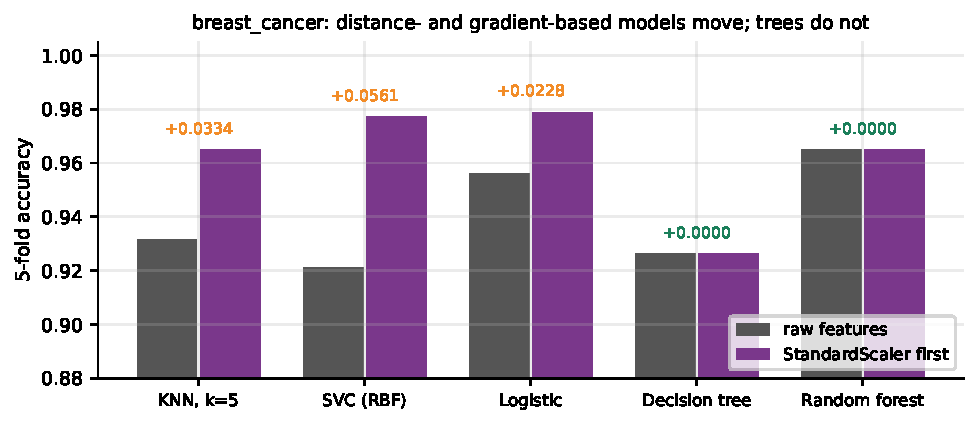
\includegraphics[width=0.80\textwidth]{scalescore.pdf}
  \end{center}
  \begin{center}\small
    Grey is raw, purple is standardised. The three left-hand pairs are the
    models that measure a distance or descend a gradient. The two right-hand
    pairs are the models that only ever ask \emph{which side of a threshold}.
  \end{center}
\end{frame}

\begin{frame}[fragile,shrink=6]{Why the tree bars are identical, exactly}
\begin{lstlisting}
t1 = DecisionTreeClassifier(random_state=0).fit(X_train, y_train)
sc = StandardScaler().fit(X_train)
t2 = DecisionTreeClassifier(random_state=0).fit(sc.transform(X_train), y_train)
\end{lstlisting}
\begin{outblk}
tree on raw    : 18 leaves, depth 5, test accuracy 0.902098
tree on scaled : 18 leaves, depth 5, test accuracy 0.902098
identical predictions on the test set: True
identical tree structure (same feature at every node): True
the thresholds differ, of course: raw 106.1000  scaled -0.0273 (same split)
\end{outblk}
\onslide<2->
\begin{center}\small
  Not ``similar'' --- \textbf{the same tree}. A split is a question about
  \emph{order}, and $x \mapsto (x-a)/b$ with $b>0$ preserves order. The
  threshold moves from $106.1$ to $-0.0273$ and separates the same patients.
\end{center}
\end{frame}

\begin{frame}[fragile,shrink=8]{Predict first \#2}
The same eight numbers $2,4,4,4,5,5,7,9$. Somebody types one extra value:
$500$.

\begin{center}
  \textbf{What happens to the eight good values under each scaler?}
\end{center}
\vspace{0.2em}
\onslide<2->
\begin{outblk}
StandardScaler  the 8 good values now span 0.0450  (was 3.5000)
MinMaxScaler    the 8 good values now span 0.0141  (was 1.0000)
RobustScaler    the 8 good values now span 2.3333  (was 4.6667)

compression factor suffered by the 8 good values
  StandardScaler    77.8 times narrower
  MinMaxScaler      71.1 times narrower
  RobustScaler       2.0 times narrower
\end{outblk}
\onslide<3->
\begin{alertblock}{$\mathbf{78\times}$, $\mathbf{71\times}$ and $\mathbf{2\times}$}
  \footnotesize The centre and width each scaler uses:
  mean $5 \to 60$, sd $2 \to 155.6$; max $9 \to 500$;
  \textbf{median $4.5 \to 5.0$ and IQR $1.5 \to 3.0$}. Only the third pair
  survived, because a median and a quartile do not care how far away a
  far-away point is.
\end{alertblock}
\end{frame}

\begin{frame}[shrink=8]{Drawn: one typo, four scalers}
  \begin{center}
    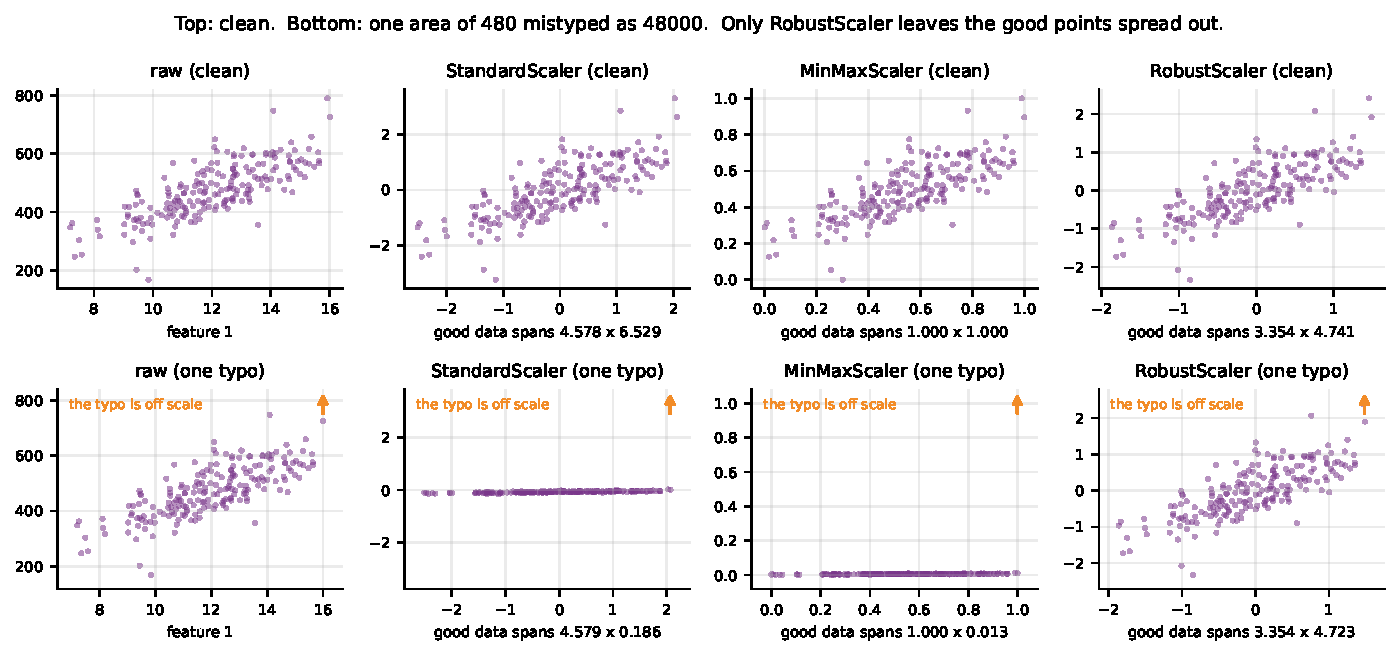
\includegraphics[width=0.92\textwidth]{scalers.pdf}
  \end{center}
  \begin{center}\small
    Two hundred plots of land; one area of $480$ typed as $48000$. The frames
    in the bottom row are the \emph{same} frames as the top row.
    \textbf{Under \texttt{MinMaxScaler} the good data occupies $1.3\%$ of the
    unit interval and every model downstream sees $200$ identical rows.}
  \end{center}
\end{frame}

\begin{frame}[fragile,shrink=8]{The gradient-based case, measured}
\texttt{SGDRegressor} on \texttt{load\_diabetes} in its original units versus
standardised. Constant step size, up to $50{,}000$ epochs.
\begin{outblk}
eta0                          raw units                 standardised
0.01              6 epochs  R2 -1.7e+28        15 epochs  R2 +0.4951
0.001             6 epochs  R2 -4.8e+26        14 epochs  R2 +0.5142
0.0001            8 epochs  R2 -4.2e+25       184 epochs  R2 +0.5144
1e-05             24 epochs  R2 +0.2008       872 epochs  R2 +0.5139
1e-06             42 epochs  R2 +0.3478      5231 epochs  R2 +0.5113
ordinary least squares on the same data gives R2 +0.5177
\end{outblk}
\onslide<2->
\begin{alertblock}{There is no step size at which the raw version works}
  \footnotesize Large steps \textbf{diverge} ($R^2 = -10^{28}$); small steps
  stop early at $0.35$. Standardised, \emph{every} step size lands within
  $0.007$ of least squares, and the best does it in \textbf{14 epochs}.
  Condition number of $X^{\!\top}\!X$: $1.03\times10^{6}$ raw against
  $470$ standardised.
\end{alertblock}
\end{frame}

\begin{frame}[shrink=8]{Drawn: the ravine}
  \begin{center}
    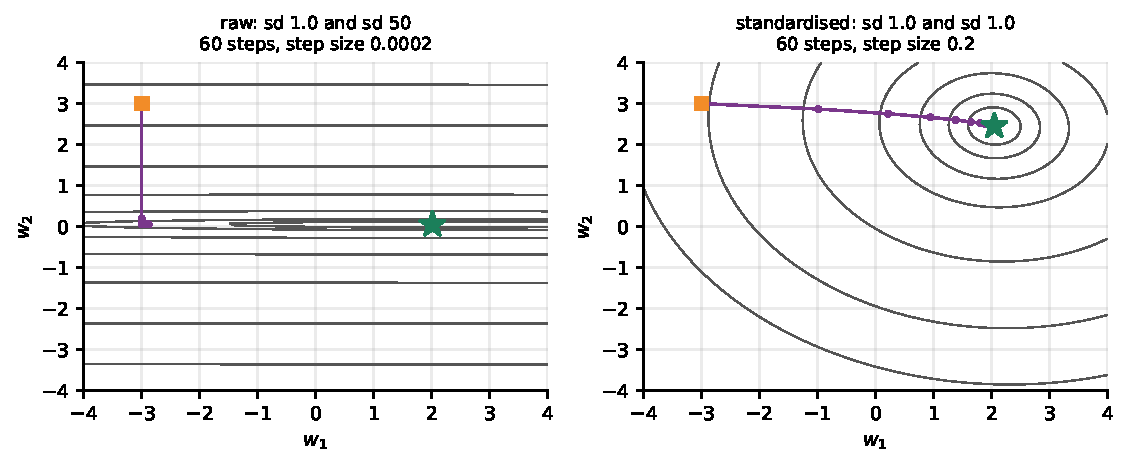
\includegraphics[width=0.80\textwidth]{gdpath.pdf}
  \end{center}
  \begin{center}\small
    Two features, one with fifty times the spread of the other. Orange square
    is the start, green star the least-squares answer. Left: the contours are
    a ravine (Hessian condition number $2296.5$) and $60$ steps end
    \textbf{$323\times$ worse than optimal}. Right: condition number $1.1$,
    and $60$ steps arrive.
  \end{center}
\end{frame}

% =====================================================================
\section[Encoding]{Feature encoding}
\label{sec:encode}

\begin{frame}[shrink=6]{A column of words is not a column of numbers}
  \begin{columns}[T]
    \begin{column}{0.48\textwidth}
      \begin{block}{Two kinds of categorical variable}
        \textbf{Ordinal} --- the categories have a real order.
        \texttt{small} $<$ \texttt{medium} $<$ \texttt{large}; a degree
        classification; a Likert scale.\\[0.4em]
        \textbf{Nominal} --- they do not. Colour, city, blood group,
        department, payment method.
      \end{block}
    \end{column}
    \begin{column}{0.48\textwidth}
      \begin{exampleblock}{Two encodings}
        \textbf{Ordinal} --- one integer column, $0, 1, 2, \dots$\\[0.3em]
        \textbf{One-hot} --- one $0/1$ column per category, exactly one of
        them $1$ in each row.
      \end{exampleblock}
      \begin{alertblock}{The decision}
        \small Match the encoding to the \emph{variable}, not to your
        convenience. Ordinal-encoding a nominal variable asserts an order
        that is not there --- and a linear model believes assertions.
      \end{alertblock}
    \end{column}
  \end{columns}
\end{frame}

\begin{frame}[shrink=8]{By hand: three colours, ordinal-coded}
  \texttt{OrdinalEncoder} sorts alphabetically:
  \texttt{blue}$\to 0$, \texttt{green}$\to 1$, \texttt{red}$\to 2$. The true
  mean target for each colour is $20$, $50$, $10$.
  \begin{center}\small
  \begin{tabular}{@{}lrrr@{}}
    \toprule
    & \texttt{blue} $=0$ & \texttt{green} $=1$ & \texttt{red} $=2$\\
    \midrule
    true mean & $20$ & $\mathbf{50}$ & $10$\\
    best straight line & $31.67$ & $26.67$ & $21.67$\\
    \bottomrule
  \end{tabular}
  \end{center}
  \vspace{0.2em}
  Least squares on three points: $\bar x = 1$, $\bar y = 26.667$,
  $S_{xy} = -10$, $S_{xx} = 2$, so slope $=-5$ and intercept $=31.667$.
  \[
    R^2 = 1 - \frac{816.7}{866.7} = \mathbf{0.0577}.
  \]
  \begin{alertblock}{The line is forced to put \texttt{green} between the others}
    \small A line through the codes $0,1,2$ \emph{cannot} put the middle
    category highest. It captures $5.8\%$ of the variation between three
    perfectly separated groups.
  \end{alertblock}
\end{frame}

\begin{frame}[fragile,shrink=6]{Predict first \#3}
$900$ rows, one nominal column, three colours with mean targets $20$, $50$
and $10$ and a noise sd of $2$. \textbf{The colour determines the target
almost exactly.}

\begin{center}
  \textbf{What cross-validated $R^2$ does a linear model get with ordinal
  coding? With one-hot?}
\end{center}
\vspace{0.2em}
\onslide<2->
\begin{outblk}
linear model, ordinal (1 column)   cross-validated R2 +0.0743
linear model, one-hot (3 columns)  cross-validated R2 +0.9868
a decision tree on the SAME ordinal column: accuracy 1.0000
\end{outblk}
\onslide<3->
\begin{alertblock}{$0.07$ against $0.99$, from a choice of encoder}
  \footnotesize The information is identical in both cases. Ordinal coding
  hid $92\%$ of it from a linear model --- and the hand calculation predicted
  $0.0577$. \textbf{Read the third line too: a tree recovers it
  perfectly, because two splits on the code column separate three groups.}
\end{alertblock}
\end{frame}

\begin{frame}[shrink=8]{Drawn: what each encoding lets the model say}
  \begin{center}
    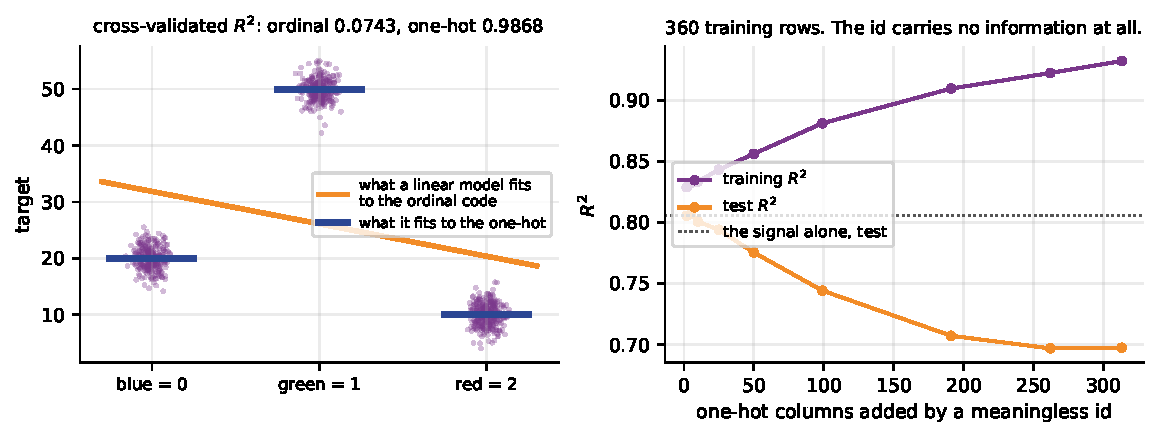
\includegraphics[width=0.94\textwidth]{encoding.pdf}
  \end{center}
  \begin{center}\small
    Left: the orange line is everything a linear model can express about an
    ordinal code; the three blue bars are what one-hot lets it say. Right:
    the price of the opposite mistake --- one-hot encoding an identifier
    that carries no information at all.
  \end{center}
\end{frame}

\begin{frame}[fragile,shrink=8]{The dummy variable trap}
Keep all three one-hot columns \emph{and} an intercept:
\begin{outblk}
with an intercept and all 3 dummies: shape (900, 4)  rank 3
   the three dummy columns sum to [1.] in every row
   condition number 3.436e+15
with an intercept and 2 dummies:     shape (900, 3)  rank 3
   condition number 3.810e+00
\end{outblk}
\onslide<2->
\begin{outblk}
coefficients, all 3 dummies : [ 19.9581   0.0382  29.926  -10.0061]
a DIFFERENT coefficient vector: [ 119.9581  -99.9618  -70.074  -110.0061]
   same predictions? max difference 8.88e-15
\end{outblk}
\onslide<3->
\begin{alertblock}{Add $c$ to the intercept, subtract $c$ from all three dummies}
  \footnotesize The predictions move by $9\times10^{-15}$, which is
  floating-point dust. There is no unique answer, so \textbf{the coefficients
  mean nothing and you must not interpret them}. Fix it with
  \texttt{drop='first'}: condition number $3.4\times10^{15} \to 3.81$. Trees and ridge do not care; least squares and
  every $p$-value do.
\end{alertblock}
\end{frame}

\begin{frame}[fragile,shrink=8]{High cardinality: one-hot on an identifier}
$600$ rows. One useful numeric feature. One customer id with $256$ distinct
values, generated at random and \textbf{carrying no information whatever}.
\begin{outblk}
the id column has 256 distinct levels in 600 rows; one-hot makes 256 columns
signal only          train R2 +0.7586   test R2 +0.8063
signal + one-hot id  train R2 +0.8956   test R2 +0.6825
levels present in train but not test: 99
\end{outblk}
\onslide<2->
\begin{columns}[T]
  \begin{column}{0.52\textwidth}
    \begin{alertblock}{Training up, test down}
      \small $+0.14$ on the training set, $-0.12$ on the test set. Each dummy
      fits a handful of rows exactly and predicts nothing.
    \end{alertblock}
  \end{column}
  \begin{column}{0.44\textwidth}
    \begin{block}{What to do instead}
      \small Group rare levels into \texttt{other}; use a target or count
      encoding fitted \emph{inside} the fold; or use a model that handles
      categories natively.
    \end{block}
  \end{column}
\end{columns}
\end{frame}

\begin{frame}[fragile,shrink=8]{Two details that will bite you in the lab}
\begin{lstlisting}
enc = OneHotEncoder().fit([["small"], ["medium"], ["large"], ["small"]])
enc.transform([["extra-large"]])
\end{lstlisting}
\begin{outblk}
OneHotEncoder() default  ->  ValueError: Found unknown categories
   [np.str_('extra-large')] in column 0 during transform
handle_unknown='ignore'  ->  all-zero row:
[[0. 0. 1.]
 [0. 0. 0.]]
\end{outblk}
\onslide<2->
\begin{lstlisting}
OrdinalEncoder().fit_transform(sizes)                      # ALPHABETICAL
OrdinalEncoder(categories=[["small","medium","large"]])     # what you meant
\end{lstlisting}
\begin{outblk}
alphabetical (the default): [2. 1. 0. 1. 2.]
   categories_ = ['large' 'medium' 'small']
stated order              : [0. 1. 2. 1. 0.]
\end{outblk}
\onslide<3->
\begin{center}\small
  \textbf{The default put \texttt{large} before \texttt{medium}.} If your
  variable really is ordinal, you must say so; the encoder cannot read
  English.
\end{center}
\end{frame}

% =====================================================================
\section[Reduction]{Data reduction concepts}
\label{sec:reduce}

\begin{frame}[shrink=6]{Han, Kamber and Pei's three kinds of reduction}
  \begin{center}\small
  \begin{tabular}{@{}lp{4.6cm}p{4.4cm}@{}}
    \toprule
    & \textbf{What it removes} & \textbf{Methods}\\
    \midrule
    \textbf{Dimensionality} & columns &
      attribute subset selection, PCA, wavelet transforms\\[4pt]
    \textbf{Numerosity} & rows, or the raw values &
      \emph{parametric}: fit a model and keep its parameters;
      \emph{non-parametric}: histograms, clustering, sampling\\[4pt]
    \textbf{Compression} & bits &
      lossless (run-length, entropy coding); lossy (PCA, wavelets again)\\
    \bottomrule
  \end{tabular}
  \end{center}
  \vspace{0.3em}
  \begin{block}{The test for all three}
    \small \textbf{The reduced dataset must support the same analysis and
    give substantially the same answer}, and the reduction itself must cost
    less than the saving. Today: dimensionality reduction (PCA) and attribute
    subset selection (feature selection), with one measurement on sampling.
  \end{block}
\end{frame}

\begin{frame}[fragile,shrink=8]{Why fewer columns, though? The curse, measured}
$500$ points spread uniformly in a cube of dimension $d$. For each point look
at its nearest and its farthest neighbour.
\begin{outblk}
    d mean dnear  mean dfar     dfar/dnear
    2     0.0232     1.0332        67.5754
   10     0.5495     1.8870         3.5278
   50     2.1608     3.5227         1.6329
  100     3.3785     4.7283         1.4004
  500     8.4293     9.7936         1.1620
 1000    12.2254    13.6046         1.1129
\end{outblk}
\onslide<2->
\begin{alertblock}{At $d = 1000$ the farthest point is $1.11\times$ as far as the nearest}
  \footnotesize Every pair of points is at very nearly the same distance, so
  ``nearest neighbour'' stops carrying information. \textbf{$k$-NN, $k$-means
  and every kernel with a distance in it degrade as $d$ grows} --- and they
  degrade quietly.
\end{alertblock}
\end{frame}

\begin{frame}[shrink=8]{Drawn: distances concentrate}
  \begin{center}
    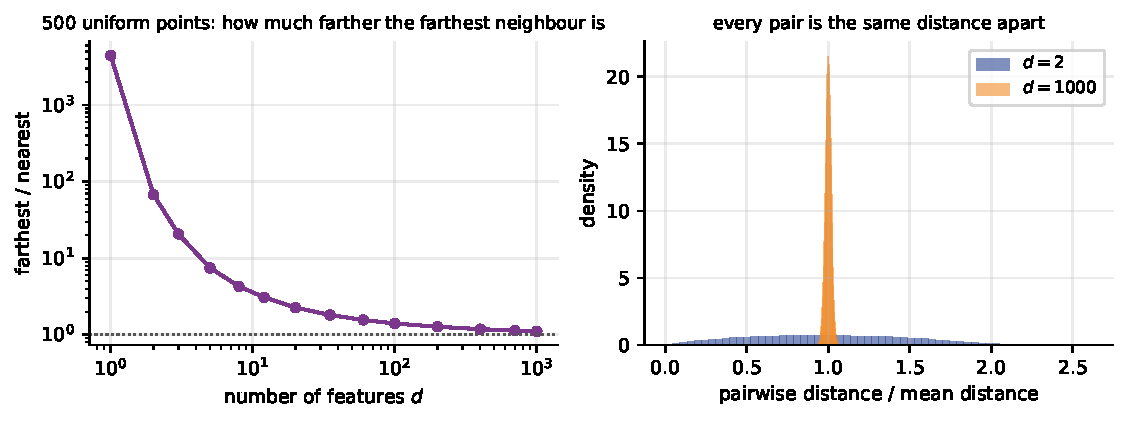
\includegraphics[width=0.88\textwidth]{curse.pdf}
  \end{center}
  \begin{center}\small
    Left: the ratio falls towards $1$ on a log--log scale. Right: the whole
    distribution of pairwise distances at $d = 2$ and $d = 1000$, each divided
    by its own mean. \textbf{At $d = 1000$ every distance in the dataset is
    within a few per cent of every other.}
  \end{center}
\end{frame}

\begin{frame}[fragile,shrink=6]{Numerosity reduction: keep fewer rows}
\texttt{load\_digits}, $1797$ rows. Take a random sample and refit.
\begin{outblk}
digits, all 1797 rows               accuracy 0.9694
digits, a   50% sample ( 898 rows)  accuracy 0.9607  loss -0.0087
digits, a   25% sample ( 449 rows)  accuracy 0.9474  loss -0.0220
digits, a   10% sample ( 179 rows)  accuracy 0.9134  loss -0.0560
digits, a    5% sample (  89 rows)  accuracy 0.8506  loss -0.1188
\end{outblk}
\onslide<2->
\begin{center}\small
  Half the data costs \textbf{under one point}. A twentieth costs twelve.
  \textbf{Sampling is the cheapest reduction there is and it is often free
  at the top of the curve} --- which is why you should prototype on a sample
  and fit on everything.
\end{center}
\onslide<3->
\begin{center}\small
  Sampling is also how you make a $200$-fold experiment finish before the
  lab ends.
\end{center}
\end{frame}

% =====================================================================
\section[PCA]{Dimensionality reduction: PCA}
\label{sec:pca}

\begin{frame}[shrink=6]{What PCA is asking}
  \begin{exampleblock}{}
    \centering
    Of all the directions in feature space, which one do the data
    \textbf{vary along the most}? Then, of the directions perpendicular to
    that one, which is next?
  \end{exampleblock}
  \vspace{0.3em}
  \begin{columns}[T]
    \begin{column}{0.48\textwidth}
      \begin{block}{The recipe}
        \begin{enumerate}\small
          \item Centre every column (subtract its mean).
          \item Form the covariance matrix
            $S = \frac{1}{n-1} X_c^{\!\top} X_c$.
          \item Take its eigenvectors and eigenvalues.
          \item Sort by eigenvalue, keep the top $k$.
        \end{enumerate}
      \end{block}
    \end{column}
    \begin{column}{0.48\textwidth}
      \begin{block}{Two facts to remember}
        \small $\lambda_j$ \emph{is} the variance along component $j$, so
        $\lambda_j / \sum_i \lambda_i$ is the fraction of variance explained.
        And $\sum_i \lambda_i = \operatorname{tr}(S)$, the total variance ---
        the rotation moves variance around but never creates or destroys it.
      \end{block}
    \end{column}
  \end{columns}
  \vspace{0.2em}
  \begin{center}\small
    Equivalently: PCA finds the $k$-dimensional subspace with the
    \textbf{smallest squared reconstruction error}. Same answer, different
    question.
  \end{center}
\end{frame}

\begin{frame}[shrink=8]{By hand: five points, three features}
  $(1,2,5),\ (2,3,4),\ (3,5,6),\ (4,4,6),\ (5,6,4)$. Mean $(3,4,5)$. Centred:
  \[
    (-2,-2,0),\ (-1,-1,-1),\ (0,1,1),\ (1,0,1),\ (2,2,-1).
  \]
  Sums of squares and products:
  $\sum x_1^2 = \sum x_2^2 = 10$, $\sum x_3^2 = 4$, $\sum x_1x_2 = 9$, and
  \textbf{$\sum x_1x_3 = \sum x_2x_3 = 0$}. Dividing by $n-1=4$:
  \[
    S = \begin{pmatrix}
      2.5 & 2.25 & 0\\ 2.25 & 2.5 & 0\\ 0 & 0 & 1
    \end{pmatrix}.
  \]
  \begin{block}{The zeros are the whole trick}
    \small $S$ is \textbf{block diagonal}: a $2\times2$ block and a scalar.
    A $3\times3$ eigenproblem would need a cubic --- this one splits into the
    $2\times2$ you already know how to do, plus the number $1$.
  \end{block}
\end{frame}

\begin{frame}[shrink=10]{The eigenvalues: $\det(S - \lambda I) = 0$}
  \[
    \det\!\begin{pmatrix}
      2.5-\lambda & 2.25 & 0\\ 2.25 & 2.5-\lambda & 0\\ 0 & 0 & 1-\lambda
    \end{pmatrix} = 0
  \]
  Expand along the third row --- its only non-zero entry is $1-\lambda$, whose
  cofactor is the top-left minor:
  \[
    (1-\lambda)\bigl[(2.5-\lambda)^2 - (2.25)^2\bigr] = 0 .
  \]
  \vspace{-0.3em}
  \begin{columns}[T]
    \begin{column}{0.47\textwidth}
      \begin{block}{First factor}
        \small $\lambda = 1$, free of charge. This is the block structure
        appearing in the algebra.
      \end{block}
    \end{column}
    \begin{column}{0.50\textwidth}
      \begin{block}{Second factor}
        \small $\lambda^2 - 5\lambda + 1.1875 = 0$, so
        \[
          \lambda = \frac{5 \pm \sqrt{20.25}}{2} = \frac{5 \pm 4.5}{2}
        \]
        $\Rightarrow\ \lambda = 4.75$ or $0.25$.
      \end{block}
    \end{column}
  \end{columns}
  \vspace{0.2em}
  \begin{alertblock}{In full: $\lambda^3 - 6\lambda^2 + 6.1875\lambda - 1.1875 = 0$}
    \footnotesize The coefficients are the invariants, so they check the roots:
    $\sum\lambda = 6 = \operatorname{tr}S$;
    $\sum_{i<j}\lambda_i\lambda_j = 6.1875$;
    $\prod\lambda = 1.1875 = \det S$.
  \end{alertblock}
\end{frame}

\begin{frame}[shrink=10]{The eigenvectors: solve $(S - \lambda I)v = 0$}
  \begin{columns}[T]
    \begin{column}{0.33\textwidth}
      \begin{block}{$\lambda_1 = 4.75$}
        \footnotesize
        $\begin{pmatrix}-2.25&2.25&0\\2.25&-2.25&0\\0&0&-3.75\end{pmatrix}$
        \smallskip

        R3: $v_3 = 0$.\\
        R1: $v_1 = v_2$.\\
        R2 repeats R1.
        \smallskip

        $u_1 = \tfrac{1}{\sqrt2}(1,1,0)$
      \end{block}
    \end{column}
    \begin{column}{0.33\textwidth}
      \begin{block}{$\lambda_2 = 1.00$}
        \footnotesize
        $\begin{pmatrix}1.5&2.25&0\\2.25&1.5&0\\0&0&0\end{pmatrix}$
        \smallskip

        Top block has\\ $\det = -2.8125 \ne 0$,\\ so $v_1 = v_2 = 0$.\\
        R3 is empty: $v_3$ free.
        \smallskip

        $u_2 = (0,0,1)$
      \end{block}
    \end{column}
    \begin{column}{0.33\textwidth}
      \begin{block}{$\lambda_3 = 0.25$}
        \footnotesize
        $\begin{pmatrix}2.25&2.25&0\\2.25&2.25&0\\0&0&0.75\end{pmatrix}$
        \smallskip

        R3: $v_3 = 0$.\\
        R1: $v_2 = -v_1$.\\
        R2 repeats R1.
        \smallskip

        $u_3 = \tfrac{1}{\sqrt2}(1,-1,0)$
      \end{block}
    \end{column}
  \end{columns}
  \vspace{0.3em}
  \begin{alertblock}{Verify, then read off the ratios}
    \footnotesize
    $S(1,1,0)^{\!\top} = (4.75,4.75,0)^{\!\top} = 4.75\,(1,1,0)^{\!\top}$ and
    $S(1,-1,0)^{\!\top} = 0.25\,(1,-1,0)^{\!\top}$. Mutually orthogonal, as a
    symmetric matrix guarantees. Ratios
    $4.75/6 = \mathbf{0.7917}$, $1/6 = 0.1667$, $0.25/6 = 0.0417$; and
    $2.5+2.5+1 = 6 = 4.75+1+0.25$ --- \textbf{nothing created, only
    rearranged}.
  \end{alertblock}
\end{frame}

\begin{frame}[shrink=8]{Drawn: the same five points}
  \begin{center}
    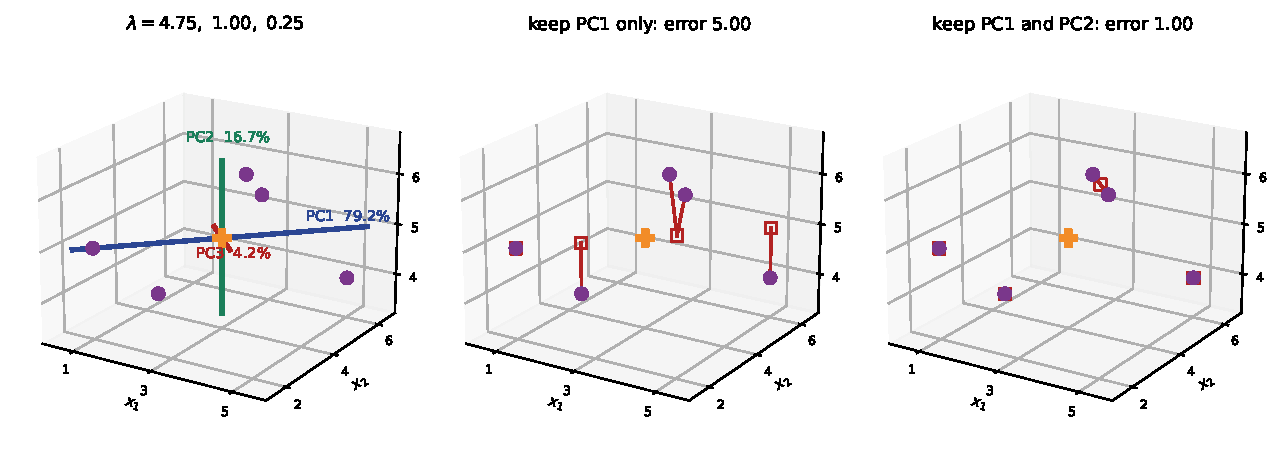
\includegraphics[width=0.94\textwidth]{pcahand.pdf}
  \end{center}
  \begin{center}\small
    Vertical axis is $x_3$. Left: the three eigenvectors at length
    $\sqrt{\lambda_j}$ --- PC2 stands straight up, because $x_3$ is
    uncorrelated with the other two and is \emph{already} a component. Middle
    and right: red squares are the reconstructions, red lines the error.
    $5.00 = 4(\lambda_2+\lambda_3)$ and $1.00 = 4\lambda_3$.
  \end{center}
\end{frame}

\begin{frame}[fragile,shrink=6]{The same thing in code}
\begin{lstlisting}
S = np.cov(P - P.mean(axis=0), rowvar=False)   # P is 5 x 3
w, V = np.linalg.eigh(S)                       # by hand
p = PCA(n_components=3).fit(P)                 # by library
\end{lstlisting}
\begin{outblk}
covariance matrix
 [[2.5  2.25 0.  ]
  [2.25 2.5  0.  ]
  [0.   0.   1.  ]]
sklearn explained_variance_       [4.75 1.   0.25]
sklearn explained_variance_ratio_ [0.791667 0.166667 0.041667]
sklearn components_ (rows)
 [[ 0.707107  0.707107  0.      ]
  [ 0.        0.        1.      ]
  [ 0.707107 -0.707107 -0.      ]]
k=1 total squared error 5.000000   check 4*(lambda2+lambda3) = 5.000000
k=2 total squared error 1.000000   check 4*lambda3          = 1.000000
\end{outblk}
\onslide<2->
\begin{center}\small
  Identical to the hand calculation, including the middle row
  $(0,0,1)$ --- the library found the same thing you did: $x_3$ is its own
  component. \textbf{And $(3,5,6)$ and $(4,4,6)$ both reconstruct to
  $(3.5, 4.5, 6)$} --- dropping a component merges points that differed only
  along it. That is what ``lossy'' means.
\end{center}
\end{frame}

\begin{frame}[fragile,shrink=8]{Predict first \#4}
Run \texttt{PCA()} on \texttt{load\_breast\_cancer} straight out of the box,
without scaling. The columns include \texttt{mean radius} (around $14$) and
\texttt{worst area} (around $880$).

\begin{center}
  \textbf{How much of the variance does the first component explain, and what
  is it?}
\end{center}
\vspace{0.2em}
\onslide<2->
\begin{outblk}
PCA on breast_cancer WITHOUT scaling
   PC1 explains 0.9820 of the variance
   its largest loading is 0.8521 on 'worst area'
   that feature's standard deviation is 568.9; the smallest in the table is 0.00264
PCA on breast_cancer WITH StandardScaler
   PC1 explains 0.4427 of the variance
   its largest loading is 0.2609 on 'mean concave points'
\end{outblk}
\onslide<3->
\begin{alertblock}{$98.2\%$ --- and it is just the area column, renamed}
  \footnotesize PCA maximises \emph{variance}, and variance has units. The
  widest column wins by construction. \textbf{Standardise before PCA unless
  every column is already in the same unit}, or you have run an expensive
  eigendecomposition to discover which column you measured in the biggest
  numbers.
\end{alertblock}
\end{frame}

\begin{frame}[fragile,shrink=6]{How many components? Read the curve}
\begin{outblk}
breast_cancer, standardised, 30 features
    1 components explain  44.27%      80% needs  5 components (16.7% of 30)
    2 components explain  63.24%      90% needs  7 components (23.3% of 30)
    5 components explain  84.73%      95% needs 10 components (33.3% of 30)
   10 components explain  95.16%      99% needs 17 components (56.7% of 30)
digits, standardised, 64 features
   80% needs 21   90% needs 31   95% needs 40   99% needs 54  of 64
\end{outblk}
\onslide<2->
\begin{alertblock}{Compare the two datasets before you generalise}
  \footnotesize breast\_cancer compresses beautifully: ten of thirty columns
  carry $95\%$, because the thirty features are ten measurements repeated
  three ways. Digits does not: \textbf{forty of sixty-four}. There is no
  universal ``keep $95\%$'' rule --- \textbf{$95\%$ of what depends entirely
  on the data}.
\end{alertblock}
\end{frame}

\begin{frame}[shrink=8]{Drawn: variance explained, and what scaling does to it}
  \begin{center}
    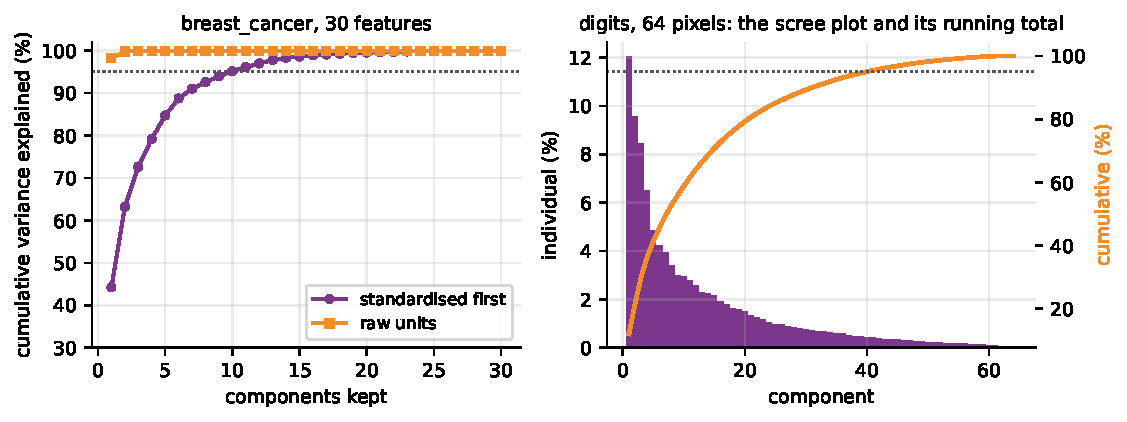
\includegraphics[width=0.90\textwidth]{pcavar.pdf}
  \end{center}
  \begin{center}\small
    Left: the orange curve starts at $98.2\%$ because one unscaled column
    dominates; the purple curve is the honest one. Right: the digits scree
    plot with its running total. \textbf{An elbow is a suggestion, not a
    criterion.}
  \end{center}
\end{frame}

\begin{frame}[fragile,shrink=6]{What you actually lose: reconstruct the digits}
Each digit is $8\times8 = 64$ pixels. Project to $k$ components and come back.
\begin{outblk}
   k= 1  variance kept  14.89%  relative reconstruction error  85.11%
   k= 2  variance kept  28.51%  relative reconstruction error  71.49%
   k= 5  variance kept  54.50%  relative reconstruction error  45.50%
   k=10  variance kept  73.82%  relative reconstruction error  26.18%
   k=20  variance kept  89.43%  relative reconstruction error  10.57%
   k=40  variance kept  98.82%  relative reconstruction error   1.18%
   k=64  variance kept 100.00%  relative reconstruction error   0.00%
\end{outblk}
\onslide<2->
\begin{center}\small
  \textbf{Variance kept and error removed add to exactly $100\%$.} That is
  not a coincidence: the reconstruction error of the top $k$ components is
  $\sum_{j>k}\lambda_j$, and dividing by $\sum_j \lambda_j$ gives
  $1 - (\text{variance kept})$.
\end{center}
\end{frame}

\begin{frame}[shrink=8]{Drawn: a digit, rebuilt from $k$ numbers}
  \begin{center}
    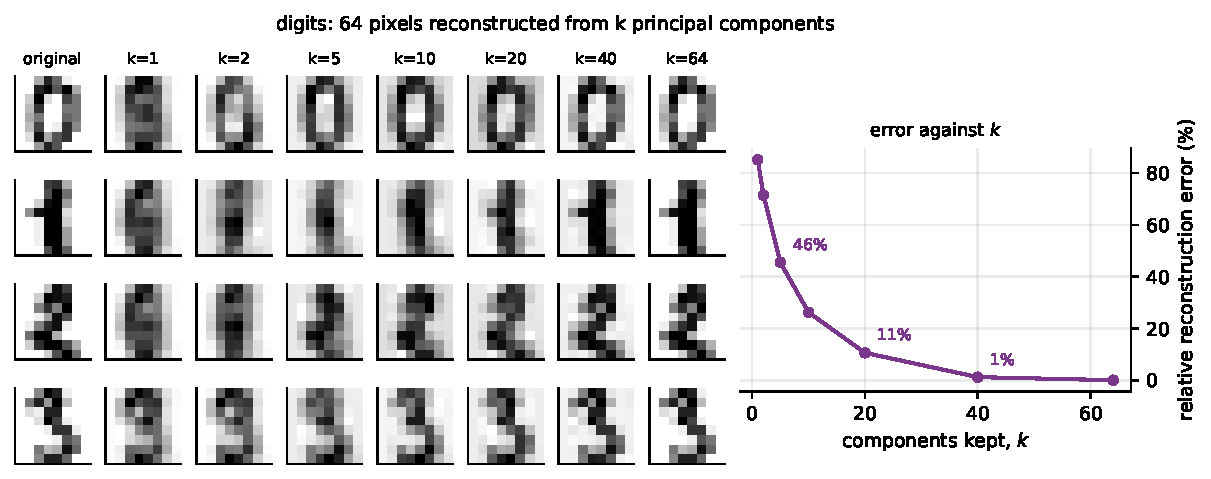
\includegraphics[width=0.98\textwidth]{pcarecon.pdf}
  \end{center}
  \begin{center}\small
    At $k = 5$ you can already tell a $0$ from a $1$; at $k = 20$ the digits
    are legible and $44$ of the $64$ numbers per image have been thrown away.
    \textbf{The error curve is the same $\sum_{j>k}\lambda_j$ read from the
    other side.}
  \end{center}
\end{frame}

\begin{frame}[fragile,shrink=8]{PCA is not feature selection}
The first component of the standardised breast\_cancer data:
\begin{outblk}
   largest  |loading| 0.2609    smallest |loading| 0.0145
   number of features with |loading| > 0.10 : 26 of 30
      +0.2609  mean concave points    +0.2584  mean concavity
      +0.2509  worst concave points   +0.2393  mean compactness
to compute PC1 for a new patient you need ALL 30 measurements.
\end{outblk}
\onslide<2->
\begin{alertblock}{Ten components does not mean ten measurements}
  \footnotesize Every component is a weighted sum of all thirty columns. You
  have reduced the \emph{width of the matrix} and not the \emph{cost of
  collecting a row}. \textbf{If your reason for reducing was ``this test is
  expensive'', PCA has not helped you at all} --- feature selection has, and
  that is the next section.
\end{alertblock}
\onslide<3->
\begin{center}\small
  And $0.2609 \times \texttt{concave points} + 0.2584 \times
  \texttt{concavity} + \dots$ is not a quantity a clinician can name.
\end{center}
\end{frame}

\begin{frame}[shrink=8]{Drawn: a mixture against a subset}
  \begin{center}
    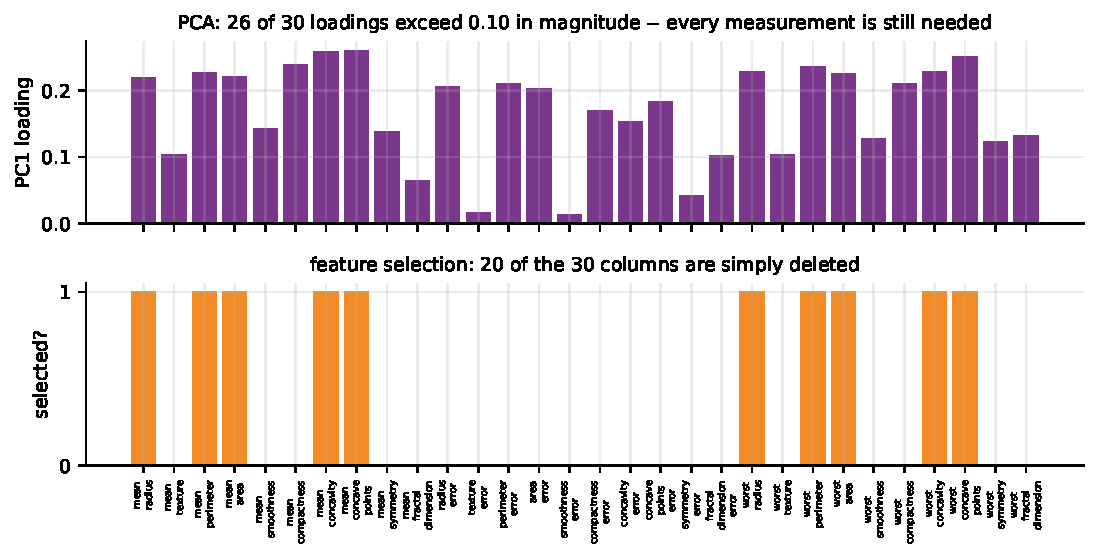
\includegraphics[width=0.86\textwidth]{pcaload.pdf}
  \end{center}
  \begin{center}\small
    Top: the thirty PC1 loadings --- twenty-six of them above $0.10$. Bottom:
    what a filter selecting ten features does to the same thirty columns.
    \textbf{One rotates; the other deletes. They are answers to different
    questions.}
  \end{center}
\end{frame}

\begin{frame}[fragile,shrink=8]{And PCA has never heard of your labels}
Two features: one with sd $10$ and no signal, one with sd $1$ that
\emph{is} the label.
\begin{outblk}
PC1 explains 0.9909 of the variance; its loadings are [1.     0.0052]
logistic regression on both features        accuracy 0.9850
logistic regression on PCA's 1 component    accuracy 0.5200
logistic regression on the 1 feature a filter would pick  0.9933
after standardising first, PCA's component  accuracy 0.7617
\end{outblk}
\onslide<2->
\begin{alertblock}{PCA threw away the answer and kept the noise}
  \footnotesize $0.9850 \rightarrow 0.5200$, which is a coin flip. PCA is
  \textbf{unsupervised}: it maximises variance, and variance is not
  relevance. A supervised filter picking one column got $0.9933$.
  \textbf{Standardising first helps ($0.7617$) but does not fix it}, because
  the problem is not the units --- it is that $y$ was never consulted.
\end{alertblock}
\end{frame}

\begin{frame}[fragile,shrink=8]{PCA is fitted on the training split. Only.}
Three ways to run the same experiment, $40$ random splits of breast\_cancer,
$10$ components:
\begin{outblk}
  correct                  accuracy 0.9768  +/- 0.0128   worst split 0.9357
  fit on everything        accuracy 0.9773  +/- 0.0122   worst split 0.9415
  refit on the test set    accuracy 0.9447  +/- 0.0226   worst split 0.8947
  fit-on-everything minus correct: +0.0006  t +0.94  wins 8/40
  components whose sign flipped between the two fits: 3.0 of 10, up to 6
\end{outblk}
\onslide<2->
\begin{alertblock}{Be honest about which of the two mistakes is which}
  \footnotesize Fitting PCA on all the rows before splitting leaked
  \textbf{nothing measurable} here ($t = 0.94$) --- PCA never sees $y$, so
  there is little to leak. Calling \texttt{fit\_transform} \emph{again} on
  the test set is a different and much worse error: $-0.0320$ on average
  and $-0.0877$ at worst, because the
  test components are a different basis --- three of the ten point the
  opposite way.
\end{alertblock}
\onslide<3->
\begin{center}\small
  \textbf{The version that leaks a great deal is coming in two slides.}
\end{center}
\end{frame}

% =====================================================================
\section[Selection]{Feature selection}
\label{sec:select}

\begin{frame}[shrink=6]{Three families, one goal}
  \begin{center}\small
  \begin{tabular}{@{}lp{4.3cm}p{3.9cm}@{}}
    \toprule
    & \textbf{How it decides} & \textbf{Cost / risk}\\
    \midrule
    \textbf{Filter} & a statistic per feature, computed once, model ignored
      --- variance, ANOVA $F$, mutual information, correlation &
      cheapest; blind to interactions and to redundancy\\[5pt]
    \textbf{Wrapper} & fit the model repeatedly and keep what helps ---
      forward selection, backward elimination, RFE &
      most expensive; can overfit the selection\\[5pt]
    \textbf{Embedded} & the model selects while it fits --- L1 (lasso), tree
      importances & nearly free; tied to that model\\
    \bottomrule
  \end{tabular}
  \end{center}
  \vspace{0.3em}
  \begin{block}{Why bother at all}
    \small Fewer columns means a cheaper model, a cheaper \emph{row} to
    collect, less overfitting --- and, unlike PCA, an answer you can read
    out loud. \textbf{Han, Kamber and Pei call this attribute subset
    selection.}
  \end{block}
\end{frame}

\begin{frame}[fragile,shrink=6]{Filter, part 1: variance}
\texttt{load\_digits}: the corner pixels of an $8\times8$ scan are always
blank.
\begin{outblk}
digits: 3 of the 64 pixels have zero variance (always the same value)
        48 of the 64 survive a variance threshold of 1.0
logistic regression on all 64 pixels          accuracy 0.9694
      threshold   0.0 keeps 61 pixels            accuracy 0.9694
      threshold   1.0 keeps 48 pixels            accuracy 0.9694
      threshold  10.0 keeps 43 pixels            accuracy 0.9683
\end{outblk}
\onslide<2->
\begin{center}\small
  \textbf{Sixteen of the sixty-four columns removed for nothing at all}, and
  twenty-one for $0.0011$. A variance filter almost never improves a score.
  What it buys is \textbf{columns} --- and a constant column is not merely useless, it breaks
  \texttt{StandardScaler} (division by zero) and any correlation you compute.
\end{center}
\end{frame}

\begin{frame}[fragile,shrink=6]{Filter, part 2: a problem built to split them}
We need a dataset where we \emph{know} the right answer. Ten features,
one thousand rows, and a label we write ourselves:
\begin{lstlisting}
a     = rng.normal(0, 1, 1000)          # enters the label linearly
b     = rng.normal(0, 1, 1000)          # enters ONLY through |b|
noise = rng.normal(0, 1, (1000, 8))     # eight columns of nothing

label = (a + 2*(abs(b) - 0.8) + rng.normal(0, 0.4, 1000)) > 0
\end{lstlisting}
\vspace{0.2em}
\begin{columns}[T]
  \begin{column}{0.48\textwidth}
    \begin{block}{Ground truth}
      \small Exactly \textbf{two} of the ten features carry signal: $a$ and
      $b$. The other eight are independent of the label by construction.
    \end{block}
  \end{column}
  \begin{column}{0.48\textwidth}
    \begin{exampleblock}{The asymmetry}
      \small Large $a$ makes class 1 more likely. For $b$ it is
      \textbf{large $|b|$} --- so $b = +2$ and $b = -2$ push the label the
      same way.
    \end{exampleblock}
  \end{column}
\end{columns}
\vspace{0.3em}
\begin{center}\small
  A good filter should rank $a$ and $b$ first and second, in some order.
\end{center}
\end{frame}

\begin{frame}[fragile,shrink=8]{Predict first \#5}
\begin{center}
  \textbf{The ANOVA $F$ test and mutual information both score all ten
  features. Where does each of them rank $b$ --- the feature we built to
  matter?}
\end{center}
\vspace{0.3em}
\onslide<2->
\begin{outblk}
feature             ANOVA F     rank  mutual info     rank
a                   317.110        1       0.1342        2
b                     0.213        8       0.2263        1
best noise            8.326        -       0.0123        -

noise columns that beat b on F: 6 of 8
\end{outblk}
\onslide<3->
\begin{alertblock}{$F$ puts the real feature \textbf{eighth of ten}}
  \footnotesize Six of the eight pure-noise columns outrank it. Mutual
  information puts it \textbf{first} --- ahead even of $a$. Two respectable
  filters, the same data, opposite verdicts.
\end{alertblock}
\end{frame}

\begin{frame}[shrink=6]{What the ANOVA $F$ statistic actually is}
\textbf{AN}alysis \textbf{O}f \textbf{VA}riance splits the total spread of one
feature into two parts: how far the \emph{group means} sit from the overall
mean, and how far the \emph{points} sit from their own group mean. Here the
groups are the classes, so $k=2$.
\vspace{-0.2em}
\[
  \underbrace{\text{SSB} = \sum_{g} n_g (\bar{x}_g - \bar{x})^2}_{\text{between, } df = k-1}
  \qquad
  \underbrace{\text{SSW} = \sum_{g}\sum_{i \in g} (x_i - \bar{x}_g)^2}_{\text{within, } df = N-k}
\]
\[
  F \;=\; \frac{\text{MSB}}{\text{MSW}}
    \;=\; \frac{\text{SSB}/(k-1)}{\text{SSW}/(N-k)}
\]
\begin{block}{Read it as a signal-to-noise ratio}
  \small The numerator is the signal --- how far apart the classes sit. The
  denominator is the noise --- how much the data scatters anyway. Dividing
  makes $F$ \textbf{scale-free}: change the units of the column and both
  halves change by the same factor, so $F$ does not move.
\end{block}
\vspace{0.1em}
\begin{center}\small
  Under the null hypothesis that every group has the same mean,
  $F \sim F(k-1,\, N-k)$ --- which is what turns a score into a $p$-value.
\end{center}
\end{frame}

\begin{frame}[fragile,shrink=6]{The same statistic, by hand}
Our thousand rows split $n_0 = 543$, $n_1 = 457$, so $df = (1, 998)$.
\begin{outblk}
a    SSB   230.0474  SSW   723.9990  MSB  230.0474  MSW  0.7254  F =  317.1099
b    SSB     0.2230  SSW  1045.7205  MSB    0.2230  MSW  1.0478  F =    0.2128

sklearn f_classif:  a 317.1099   b 0.2128
p-values         :  a 8.201e-62   b 0.6447
\end{outblk}
\vspace{0.2em}
\begin{columns}[T]
  \begin{column}{0.48\textwidth}
    \begin{exampleblock}{$a$: enormous}
      \small The class means are far apart relative to the scatter, so
      SSB is large. $p \approx 10^{-62}$.
    \end{exampleblock}
  \end{column}
  \begin{column}{0.48\textwidth}
    \begin{alertblock}{$b$: indistinguishable from nothing}
      \small SSB is $0.2230$ out of a total of nearly $1046$. $p = 0.6447$ ---
      the test cannot reject ``no difference''.
    \end{alertblock}
  \end{column}
\end{columns}
\vspace{0.2em}
\begin{center}\small
  Four lines of arithmetic reproduce \texttt{f\_classif} exactly. Nothing is
  hidden in the library --- which is why we can say precisely what it misses.
\end{center}
\end{frame}

\begin{frame}[shrink=6]{Why $F$ is blind: it only ever compares means}
Look again at the numerator. It contains $\bar{x}_g$ and nothing else ---
\textbf{only the group means enter the signal term.} So look at where the
groups sit.
\vspace{0.2em}
\begin{center}\small
  \begin{tabular}{@{}lrrrr@{}}
    \toprule
    feature & mean $\mid y{=}0$ & mean $\mid y{=}1$ & difference & $F$\\
    \midrule
    $a$   & $-0.4880$ & $0.4748$ & $\mathbf{0.9628}$ & $317.110$\\
    $b$   & $0.0057$  & $-0.0243$ & $-0.0300$ & $0.213$\\
    \bottomrule
  \end{tabular}
\end{center}
\vspace{0.2em}
\begin{alertblock}{The signal is in the \emph{spread}, and $F$ divides it away}
  \footnotesize $b$'s two class means differ by $0.03$ --- nothing. But its
  class standard deviations are $\mathbf{0.6199}$ and $\mathbf{1.3552}$, a
  factor of $\mathbf{2.19}$. That difference is real and it is exactly what
  the \emph{denominator} of $F$ averages away. The test is not broken; it is
  answering the question it was built to answer.
\end{alertblock}
\end{frame}

\begin{frame}[shrink=8]{Drawn: the same fact, three ways}
\begin{center}
  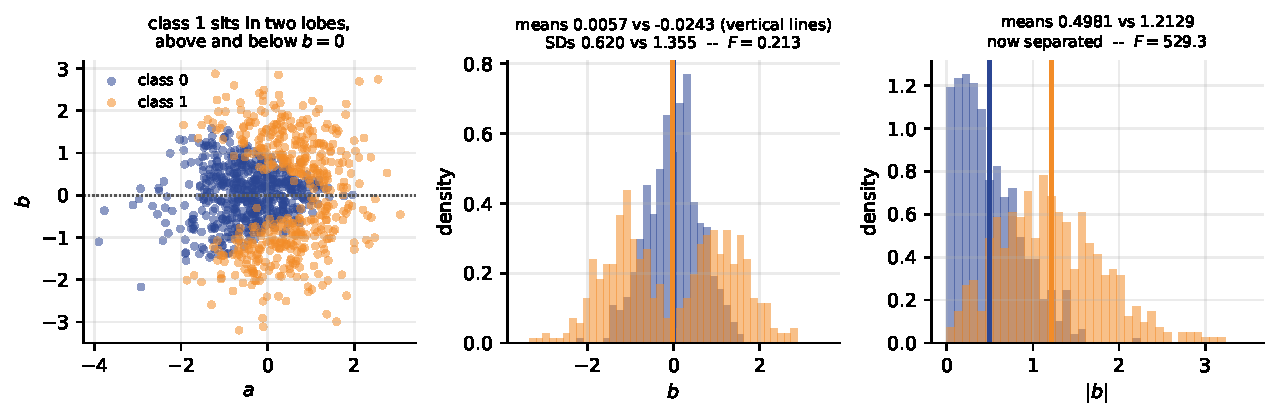
\includegraphics[width=0.96\textwidth]{filterdisagree.pdf}
\end{center}
\begin{center}\small
  Middle: the two vertical lines are the class means of $b$ --- they sit on
  top of each other, while the orange distribution is more than twice as
  wide. That picture is what $F = 0.213$ is describing. Right: take
  $|b|$ instead and the means separate at once.
\end{center}
\end{frame}

\begin{frame}[fragile,shrink=6]{What mutual information does instead}
\[
  I(X; Y) \;=\; \sum_{x}\sum_{y} p(x,y)\,
  \log\frac{p(x,y)}{p(x)\,p(y)}
\]
It measures how far the joint distribution is from the product of the
marginals --- that is, \textbf{how much knowing $X$ reduces your uncertainty
about $Y$}. It never assumes a line, a mean shift, or a direction.
\begin{outblk}
k=2   F picks ['a', 'n2']                MI picks ['a', 'b']
k=3   F picks ['a', 'n1', 'n2']          MI picks ['a', 'b', 'n8']
k=4   F picks ['a', 'n1', 'n2', 'n7']    MI picks ['a', 'b', 'n7', 'n8']
\end{outblk}
\begin{columns}[T]
  \begin{column}{0.48\textwidth}
    \begin{block}{The price}
      \small MI is estimated from neighbour distances, so it is
      \textbf{stochastic} --- pass \texttt{random\_state} or your ranking
      changes between runs --- and needs more rows than $F$ does.
    \end{block}
  \end{column}
  \begin{column}{0.48\textwidth}
    \begin{alertblock}{At every $k$}
      \small $F$ spends its budget on noise and never buys $b$. MI buys both
      real features first, then noise.
    \end{alertblock}
  \end{column}
\end{columns}
\end{frame}

\begin{frame}[fragile,shrink=8]{But which filter was actually right?}
Before declaring $F$ the loser --- feed each selection to a model and measure.
\begin{outblk}
a alone,                logistic       0.7160
a + b,                  logistic       0.7100
a + 2 noise (F's k=3),  logistic       0.7130
a + b,                  tree           0.8740
a + |b|,                logistic       0.9120
\end{outblk}
\onslide<2->
\begin{alertblock}{Adding the ``real'' feature made logistic regression
  \emph{worse}}
  \footnotesize $0.7160 \rightarrow 0.7100$. A linear model cannot use $b$ ---
  it can only fit a coefficient on $b$ itself, and the best such coefficient
  is zero. So for logistic regression, \textbf{$F$'s verdict was correct}. Give
  the same two columns to a tree, which can split twice, and accuracy jumps to
  $0.8740$.
\end{alertblock}
\end{frame}

\begin{frame}[fragile,shrink=6]{The resolution, and the lesson}
\begin{outblk}
feature             ANOVA F     rank  mutual info     rank
a                   317.110        2       0.1342        2
|b|                 529.299        1       0.2122        1
\end{outblk}
\vspace{0.1em}
Engineer the feature the problem is actually about and $F$ finds it
instantly: \textbf{$0.213 \rightarrow 529.299$, rank $8 \rightarrow$ rank 1}.
And logistic regression on $(a, |b|)$ scores $\mathbf{0.9120}$, beating the
tree.
\vspace{0.3em}
\begin{alertblock}{Three things to take away}
  \footnotesize
  \textbf{1.} A filter measures the kind of dependence it was built to
  measure, and nothing else. $F$ sees mean shifts; MI sees any dependence.\\
  \textbf{2.} ``Useful'' is not a property of a column alone --- it is a
  property of \textbf{column and model together}. $b$ is useless to a linear
  model and valuable to a tree.\\
  \textbf{3.} A disagreement between two filters is not a nuisance to be
  resolved by picking a favourite. It is \textbf{information}: it says the
  dependence is there but not of the shape one of them assumes --- which is a
  hint to go and engineer a better feature.
\end{alertblock}
\end{frame}

\begin{frame}[fragile,shrink=8]{Wrapper: recursive feature elimination}
Fit the model. Drop the feature with the smallest coefficient. Refit. Repeat.
Thirty features with \texttt{step=1} means \textbf{thirty model fits}.
\begin{outblk}
elimination order, first six      the last one standing: worst area
   dropped 30 of 30: worst compactness      dropped 27: mean smoothness
   dropped 29 of 30: mean symmetry          dropped 26: texture error
   dropped 28 of 30: concavity error        dropped 25: concave points error
   RFE k= 1  accuracy 0.9157      RFE k=10  accuracy 0.9684
   RFE k= 2  accuracy 0.9526      RFE k=20  accuracy 0.9789
   RFE k= 5  accuracy 0.9684      RFE k=30  accuracy 0.9789
   RFECV picks its own k: 26 features, accuracy 0.9824
\end{outblk}
\onslide<2->
\begin{center}\small
  A wrapper asks the \emph{model} what it needs, so it can see redundancy a
  filter cannot --- but it pays a model fit per step, and its answer is
  \textbf{that model's} answer. \textbf{Left to choose $k$ for itself,
  \texttt{RFECV} keeps $26$ of the $30$.}
\end{center}
\end{frame}

\begin{frame}[shrink=8]{Before the lasso: what an L1 or L2 penalty does}
  \small A linear model predicts
  $\hat y = w_0 + w_1 x_1 + \dots + w_d x_d$; each $w_j$ is a
  \textbf{coefficient} (weight). \textbf{If $w_j = 0$, feature $j$ is not used
  at all} --- so counting the non-zero coefficients counts the features kept.
  \begin{columns}[T]
    \begin{column}{0.49\textwidth}
      \begin{block}{Ridge --- the L2 penalty}
        \small
        \[ \min_w \; \sum_i (y_i - \hat y_i)^2 + \alpha \sum_j w_j^2 \]
        Squares get tiny near zero, so the pull fades as $w_j$ shrinks:
        weights get \emph{smaller}, almost never exactly $0$.
      \end{block}
    \end{column}
    \begin{column}{0.49\textwidth}
      \begin{block}{Lasso --- the L1 penalty}
        \small
        \[ \min_w \; \sum_i (y_i - \hat y_i)^2 + \alpha \sum_j |w_j| \]
        $|w_j|$ charges the same per unit however small $w_j$ is, so weak
        features are pushed \emph{all the way to $0$}.
      \end{block}
    \end{column}
  \end{columns}
  \begin{itemize}
    \item \textbf{$\alpha$} is the penalty strength: $\alpha = 0$ is plain least
      squares; larger $\alpha$ shrinks harder. A \textbf{path of $\alpha$} is
      the same model refitted at several values.
    \item \textbf{Embedded} selection: the features are chosen \emph{by the
      fit itself}, not by a separate filter or wrapper step.
    \item \textbf{Standardise first}: the penalty compares $|w_j|$ across
      features, which is only fair when they share a scale.
  \end{itemize}
  \footnotesize Lecture~12 treats ridge and lasso in full; here we only use
  the lasso as a selector.
\end{frame}

\begin{frame}[shrink=8]{The data on the next slide: \texttt{load\_diabetes}}
  \small $442$ patients; the target is a measure of how far the disease has
  progressed one year after these baseline readings.
  \begin{center}\small
  \begin{tabular}{@{}ll@{\qquad}ll@{}}
    \toprule
    \texttt{age} & age in years & \texttt{s1} & total serum cholesterol\\
    \texttt{sex} & sex & \texttt{s2} & LDL (``bad'') cholesterol\\
    \texttt{bmi} & body mass index & \texttt{s3} & HDL (``good'') cholesterol\\
    \texttt{bp}  & average blood pressure & \texttt{s4} & total cholesterol / HDL\\
    & & \texttt{s5} & log of serum triglycerides\\
    & & \texttt{s6} & blood sugar level\\
    \bottomrule
  \end{tabular}
  \end{center}
  \begin{block}{How to read each row of the output}
    \small \textbf{nonzero} = coefficients the lasso left non-zero, i.e.\ the
    features it kept (named when there are few).
    \textbf{CV R2} = mean $R^2$ over $5$-fold cross-validation, scaler and
    lasso refitted inside each fold. Higher is better; $1$ is perfect.
  \end{block}
\end{frame}

\begin{frame}[fragile,shrink=6]{Embedded: L1 chooses by shrinking to zero}
Lasso on \texttt{load\_diabetes}, standardised, over a path of $\alpha$:
\begin{outblk}
   alpha  0.01  10 nonzero  CV R2 +0.4823
   alpha  0.50   8 nonzero  CV R2 +0.4818
   alpha  1.00   7 nonzero  CV R2 +0.4820
   alpha  5.00   5 nonzero  CV R2 +0.4659  sex,bmi,bp,s3,s5
   alpha 20.00   3 nonzero  CV R2 +0.3492  bmi,bp,s5
   ridge alpha 1.00  10 nonzero  CV R2 +0.4822
\end{outblk}
\onslide<2->
\begin{center}\small
  \textbf{Three of ten features keep $72\%$ of the $R^2$; five of ten keep
  $97\%$.} The lasso gives you the whole trade-off curve for free, and
  \textbf{$\alpha$ is the dial}. Ridge ($\alpha = 1$) keeps all ten and
  scores the same --- L1 selects, L2 only shrinks.
\end{center}
\onslide<3->
\begin{center}\small
  Selection here is $\alpha$-dependent, so it is a hyper-parameter and belongs
  inside the cross-validation loop like any other.
\end{center}
\end{frame}

\begin{frame}[fragile,shrink=8]{All four on the same data --- and they disagree}
Ten features of thirty, \texttt{load\_breast\_cancer}:
\begin{outblk}
pairwise overlap (Jaccard)
   ANOVA F       vs mutual info    9 shared, Jaccard 0.82
   ANOVA F       vs RFE            6 shared, Jaccard 0.43
   ANOVA F       vs L1 logistic    4 shared, Jaccard 0.29
   RFE           vs L1 logistic    6 shared, Jaccard 0.50
chosen by all four: mean concave points, worst radius, worst concave points
chosen by at least one: 16 of 30 features
\end{outblk}
\onslide<2->
\begin{alertblock}{Three features out of thirty command a consensus}
  \footnotesize The two filters agree with each other ($0.82$) and with
  nobody else. \textbf{There is no such thing as ``the important features''}
  --- there is only ``the features this criterion, with this model, at this
  $k$, chose''. Report the criterion whenever you report a selection.
\end{alertblock}
\end{frame}

\begin{frame}[fragile,shrink=6]{Does selection actually help? Measure it}
\begin{outblk}
selector                   accuracy
all 30 features              0.9789
filter: ANOVA F, k=10        0.9596
filter: mutual info, k=10    0.9561
wrapper: RFE, k=10           0.9684
embedded: L1, C=0.08         0.9719
\end{outblk}
\onslide<2->
\begin{alertblock}{On this dataset, every selector lost accuracy}
  \footnotesize Not one of the four beat simply using all thirty columns.
  RFE, at $21$ model fits per fold against a filter's $1$, recovered the
  most. \textbf{Do
  not select because you were told to.} Select when you need a cheaper row,
  a readable model, or when $d$ is large relative to $n$ --- which
  breast\_cancer, at $569 \times 30$, is not.
\end{alertblock}
\onslide<3->
\begin{center}\small
  Reporting the experiment that did \emph{not} work is part of doing the
  experiment.
\end{center}
\end{frame}

\begin{frame}[fragile,shrink=8]{Predict first \#5}
$500$ features, $60$ rows, all of it drawn from $\mathcal{N}(0,1)$. The labels
are \textbf{coin flips}. There is nothing to learn: the honest answer is
$0.5$.

Now do what everyone does: compute the ANOVA $F$ of every feature
\emph{on all the data}, keep the best $20$, and cross-validate on those.

\begin{center}
  \textbf{What accuracy comes out?}
\end{center}
\vspace{0.2em}
\onslide<2->
\begin{outblk}
   select on ALL the data, then cross-validate : 0.8475  +/- 0.0293
   select INSIDE each fold (Pipeline)          : 0.5342  +/- 0.0710
   overstatement                                +0.3133
   the wrong way beat 0.5 on 20 of 20 repetitions
\end{outblk}
\onslide<3->
\begin{alertblock}{$0.85$ on data that contains no information at all}
  \footnotesize With $500$ candidates and $60$ rows, some feature correlates
  with the labels by luck --- and you \emph{chose it using the labels of the
  rows you are about to test on}. Every fold's ``held-out'' rows had already
  voted. \textbf{$+0.31$, on twenty repetitions out of twenty.}
\end{alertblock}
\end{frame}

\begin{frame}[shrink=8]{Drawn: what each selector picks, and the leak}
  \begin{center}
    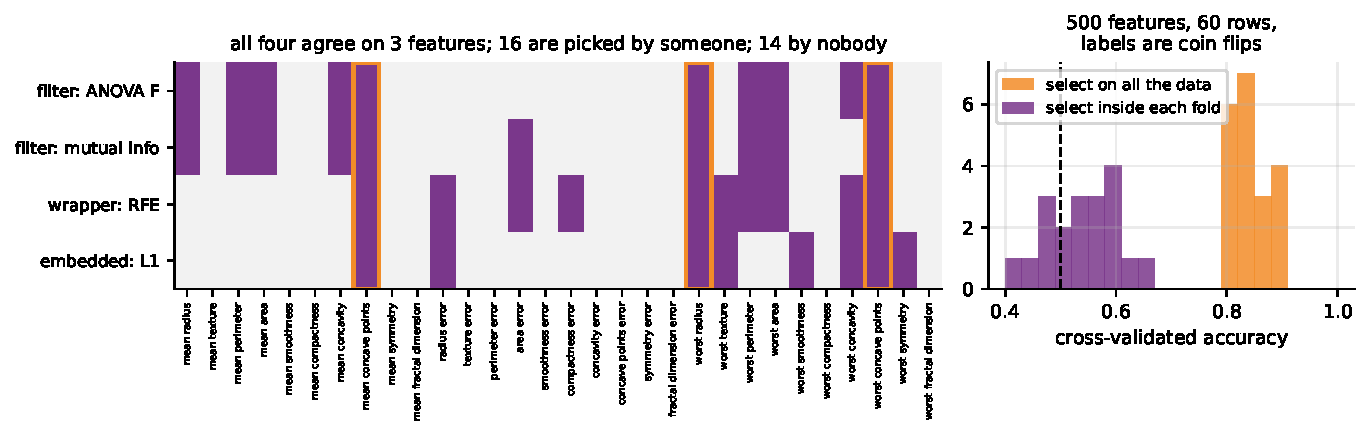
\includegraphics[width=0.98\textwidth]{selection.pdf}
  \end{center}
  \begin{center}\small
    Left: the four selectors against the thirty features; orange boxes mark
    unanimity. Right: the two histograms are the \emph{same experiment} on
    the \emph{same random data}, differing only in whether the selector was
    fitted inside the fold. The dashed line is the truth.
  \end{center}
\end{frame}

% =====================================================================
\section{Summary}
\label{sec:summary}

\begin{frame}[fragile,shrink=4]{The pipeline that cannot leak}
\begin{lstlisting}
pipe = Pipeline([
    ("scale",  StandardScaler()),
    ("select", SelectKBest(f_classif, k=15)),
    ("pca",    PCA(n_components=8)),
    ("model",  LogisticRegression(max_iter=5000)),
])
cross_val_score(pipe, X, y, cv=5).mean()
\end{lstlisting}
\begin{outblk}
scale -> select 15 -> PCA to 8 -> logistic regression
   5-fold accuracy 0.9490  +/- 0.0140
   compare: raw logistic regression, all 30 features 0.9789
\end{outblk}
\onslide<2->
\begin{center}\small
  The mean, the standard deviation, the fifteen chosen columns and the eight
  rotations are all recomputed inside every fold, from four fifths of the
  data. \textbf{And note the second line: the four-step pipeline is worse
  than doing nothing.} It cannot leak, and it also did not help.
\end{center}
\end{frame}

\begin{frame}[shrink=15]{Summary --- twelve lines}
  \begin{enumerate}\small
    \item A representation is good only relative to a model. One product
      column took a linear model from $R^2 = 0.9091$ to $0.9981$; a tree got
      there unaided.
    \item Binning gained the linear model $+0.0957$ and cost the tree
      $-0.0323$ --- and made both fit exactly the same function.
    \item \texttt{PolynomialFeatures} degree $3$ turns $30$ columns into
      $5455$; on diabetes, degree $2$ cost $-0.0643$ of $R^2$.
    \item Age against income: the income column supplied $99.995\%$ of the
      squared distance, and standardising \textbf{changed which customer was
      the nearest neighbour}.
    \item Scaling was worth $+0.0561$ to an RBF SVM, $+0.0334$ to $k$-NN,
      $+0.0246$ to logistic regression, and \textbf{exactly $0.0000$} to a
      tree and a forest --- the same tree, node for node.
    \item Unscaled, gradient descent diverged at every usable step size.
      Standardised, it reached least squares in $14$ epochs.
    \item One typo squeezed the good data $78\times$ under
      \texttt{StandardScaler}, $71\times$ under \texttt{MinMaxScaler}, and
      $2\times$ under \texttt{RobustScaler}.
    \item Ordinal-coding a nominal variable: $R^2 = 0.0743$ against $0.9868$
      for one-hot. The hand calculation predicted $0.0577$.
    \item Intercept plus all $k$ dummies is rank-deficient: condition number
      $3.4\times10^{15}$, and two completely different coefficient vectors
      give identical predictions.
    \item PCA on unscaled data: PC1 explained $98.20\%$ and was the widest
      column. Standardised: $44.27\%$, and $95\%$ needed $10$ of $30$
      components (but $40$ of $64$ on digits).
    \item PCA is a rotation, not a selection --- $26$ of $30$ loadings exceed
      $0.10$ --- and it is unsupervised: it took an accuracy of $0.9850$ down
      to $0.5200$ by discarding the only informative direction.
    \item \textbf{Selecting features on all the data before cross-validating
      scored $0.8475$ on pure coin flips.} Inside a \texttt{Pipeline}:
      $0.5342$.
  \end{enumerate}
\end{frame}

\begin{frame}[shrink=3]{Before the next lecture}
  \begin{columns}[T]
    \begin{column}{0.48\textwidth}
      \begin{block}{Read}
        \texttt{notes.pdf} --- the full eigen-decomposition worked by hand,
        the reconstruction-error identity, and \textbf{10 practice questions
        with worked solutions}.
      \end{block}
      \begin{block}{Do}
        Questions 3, 6 and 9. Question 6 is PCA on a $2\times2$ covariance
        matrix by hand; question 9 is a debugging story you will meet for
        real.
      \end{block}
    \end{column}
    \begin{column}{0.48\textwidth}
      \begin{exampleblock}{Next: splitting and validation}
        Train/test strategies, cross-validation, and imbalanced data. Carry
        one thing across: \textbf{the last slide of this lecture is the first
        slide of that one.}
      \end{exampleblock}
      \begin{alertblock}{And a habit to start now}
        Every preprocessing step goes in the \texttt{Pipeline}. If you find
        yourself calling \texttt{fit\_transform} on \texttt{X} before
        splitting, stop and ask what that step just learned.
      \end{alertblock}
    \end{column}
  \end{columns}
  \begin{center}
    \small Materials: \texttt{\AMLRepoURL}
  \end{center}
  \slidesources{\AMLUnitIVSources}
\end{frame}

\end{document}
